\documentclass[a4paper,
DIV=13,
12pt,
BCOR=10mm,
department=FakEI,
%lucida,
%KeepRoman,
oneside,
parskip=half,
automark,
%headsepline,
]{OTHRartcl}
\usepackage[ngerman]{babel}
\usepackage[T1]{fontenc}
\usepackage[utf8]{inputenc}
\usepackage{lmodern}

\usepackage{subcaption}
\usepackage{wrapfig,graphicx}
\usepackage{placeins}
\usepackage{amsmath}
\usepackage{amsfonts}
\usepackage{dsfont}
\usepackage{enumerate}
\usepackage{graphicx}
\usepackage{mathrsfs}
\usepackage{braket}
\usepackage{color}
\usepackage[colorlinks=true, linkcolor=cyan]{hyperref}
\usepackage[ugly]{units}

\usepackage{marvosym}
%\usepackage{hyperref}
%\hypersetup{
%	colorlinks = true,
%	linkcolor = cyan,
%	urlcolor = cyan
%}
% Default fixed font does not support bold face
\DeclareFixedFont{\ttb}{T1}{txtt}{bx}{n}{12} % for bold
\DeclareFixedFont{\ttm}{T1}{txtt}{m}{n}{12}  % for normal

\let\oldunit\unit
\renewcommand{\unit}[1]{\oldunit{\,#1}}
\renewcommand{\phi}{\varphi}
\newcommand{\diff}{\text{d}}
\renewcommand{\vec}[1]{\mathbf{#1}}

%\usepackage[singlelinecheck=off]{caption}
\setkomafont{captionlabel}{\bfseries}
\renewcommand*{\captionformat}{.~~}
\setcapindent{0pt}
\addto\captionsngerman{\renewcommand\figurename{Abb.}}


\usepackage{listings,xcolor}
\renewcommand{\lstlistingname}{Programmcode}
% Custom colors
\definecolor{pl_background}{rgb}{0.95,0.95,0.95}
\definecolor{pl_comment}{rgb}{0.12, 0.38, 0.18 }
\definecolor{pl_ifelse}{rgb}{0.74,0.74,.29}
\definecolor{pl_keyword}{rgb}{0.37, 0.08, 0.25}
\definecolor{pl_string}{rgb}{0.06, 0.10, 0.98}
\definecolor{deepblue}{rgb}{0,0,0.5}
\definecolor{deepred}{rgb}{0.6,0,0}
\definecolor{deepgreen}{rgb}{0,0.5,0}

% Vordefiniertes Programmlisting
\lstset{
	language = C,
	basicstyle = \small\sffamily,
	backgroundcolor = \color{pl_background},
	stringstyle = \color{pl_string},
	keywordstyle = \color{pl_keyword}\bfseries,
	commentstyle = \color{pl_comment}\itshape,
	frame = lrbt,
	numbers = left,
	showstringspaces = false,
	breaklines = true,
	xleftmargin = 15pt,
	emph = [1]{php},
	emphstyle = [1]\color{black},
	emph = [2]{if,and,or,else},
	emphstyle = [2]\color{pl_ifelse}
}

\lstset{
	language = Matlab,
	basicstyle = \small\sffamily,
	backgroundcolor = \color{pl_background},
	stringstyle = \color{pl_string},
	keywordstyle = \color{pl_keyword}\bfseries,
	commentstyle = \color{pl_comment}\itshape,
	frame = lrbt,
	numbers = left,
	showstringspaces = false,
	breaklines = true,
	xleftmargin = 15pt,
	emph = [1]{php},
	emphstyle = [1]\color{black},
	emph = [2]{if,and,or,else},
	emphstyle = [2]\color{pl_ifelse},
	tabsize=4
}

% Python style for highlighting
\newcommand{\pythonstyle}{\lstset{
		language=Python,
		basicstyle=\ttm,
		numbers = left,
		otherkeywords={self},             % Add keywords here
		keywordstyle=\ttb\color{deepblue},
		emph={MyClass,__init__},          % Custom highlighting
		emphstyle=\ttb\color{deepred},    % Custom highlighting style
		stringstyle=\color{deepgreen},
		backgroundcolor = \color{pl_background},
		breaklines = true,
		xleftmargin = \parindent,
		tabsize = 4,					% Aendert tab einzug, muss aber mit gobble abgestimmt werden
		gobble = 7,
		showstringspaces=false            % 
}}

\newcommand{\bashstyle}{\lstset{
		language = bash,
		basicstyle=\ttm,
		numbers = left,
		otherkeywords={self},             % Add keywords here
		keywordstyle=\ttb\color{deepblue},
		stringstyle=\color{deepgreen},
		backgroundcolor = \color{pl_background},
		breaklines = true,
		xleftmargin = \parindent,
		tabsize = 4,					% Aendert tab einzug, muss aber mit gobble abgestimmt werden
		gobble = 7,
		showstringspaces=false  					
}}

% Python environment
\lstnewenvironment{python}[1][]
{
	\renewcommand{\lstlistingname}{Code}
	\pythonstyle
	\lstset{#1}
}
{}
\lstnewenvironment{bash}[1][]
{
	\renewcommand{\lstlistingname}{Code}
	\bashstyle
	\lstset{#1}
}{}

\pagestyle{headings}
\usepackage{lipsum}

%remove all empty pages
\renewcommand\cleardoublepage{%
	\clearpage
	\ifodd\value{page}\else\stepcounter{page}\fi
}
\usepackage[backend=bibtex, style=numeric-comp, sorting=none]{biblatex}
\bibliography{bib}
%\title{Intelligentes Schuhwerk für den humanoiden NAO Roboter basierend auf Magnetostiction zur Verbesserung der Bodenhaftung}
\title{Entwicklung eines magneto-aktiven Schuhwerks für den humanoiden NAO Roboter zur Verbesserung der Gangstabilität}
\author{Tamara Szecsey}
\documenttype{Masterarbeit}

\studentid{3140789}
\department{Elektro- und Informationstechnik}
\studyprogramme{Master Electrical- and Microsystem Engineering}
\startingdate{1.\,Juni 2020}
\closingdate{31.\,März 2021}

\firstadvisor{Prof. Dr. Gareth Monkman}
\secondadvisor{Dr. Dirk Sindersberger}
%\externaladvisor{Dr. Klara Endlos}
\externallogo[height=1.6cm]{Bilder/mru.png}

\begin{document}
%	\numberwithin{equation}{section}
\maketitle
%\cleardoublepage
\makedeclaration

\thispagestyle{empty}
\tableofcontents	
\clearpage	
\setcounter{page}{1}

\section{Einleitung}
%* über humanoide Roboter (Vor- und Nachteile) \\
%* über nao und seine beschaffenheit \\
%* über map \\
%* Ziel der Arbeit \\
%* magnetostiction
%
%* Aufbau des Schuhs
%* 
Kapitel \ref{kap_MAP} erklärt die Definition und Eigenschaften von Magneto-aktiven Polymeren (MAP), welche als Sohle für den Nao Roboter eingesetzt wurden. Diese Erklärungen basieren auf einem Buch von Pelteret und Steinmann \cite{map2020}, welches ich für tiefergehende Lektüren empfehle. 
\newpage
\section{Theoretischer Hintergrund}
\subsection{Aufbau des NAO} \label{aufbau_NAO}
%* zu softbank robotics
%* allgemeines zur größe, zu den freiheitsgraden und den Sensoren
%* Genaueres zu den Sensoren, die gemessen wurden
%* Grenzen des Naos

\begin{wrapfigure}{hr}{0.3\linewidth}
	\vspace{-1cm}
	\centering
	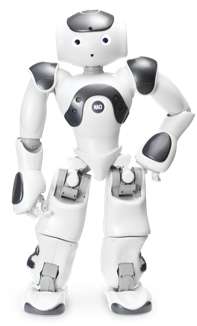
\includegraphics[width=\linewidth]{Bilder/naov6.png}
	\caption{NAO V6 \cite{nao_docu_dev_guide}}
	\label{nao_v6}
	\vspace{-2cm}
\end{wrapfigure}
NAO ist ein $574 \unit{mm}$ großer, humanoider Roboter (siehe Abb. \ref{nao_v6}) ursprünglich entwickelt von dem französischen Unternehmen Aldeberan Robotics, welche 2015 von Softbank Group aufgekauft \cite{aldebaran_to_softbank} und in Softbank Robotics umbenannt wurde. Während NAO's große Schwester Pepper mit ihren $1,20 \unit{m}$ mit einem Tablet und Rollen statt Beinen ausgestattet ist \cite{about_pepper}, gibt es NAO in verschiedenen Ausführungen, sowohl ab der Hüfte aufwärts als auch mit Beinen. Es handelt sich hier um Roboter, die unter anderem Kindern und Jugendlichen die Robotik näher bringen sollen und der Vorführung von Mensch-Roboter Interaktionen dienen. NAO bietet außerdem die Gelegenheit zweibeinige Robotersysteme zu studieren und ist bereits in psychologischen Studien verwendet worden \cite{SHAMSUDDIN20121533}. 

\begin{figure}[hb]
	\centering
	\vspace{2cm}
	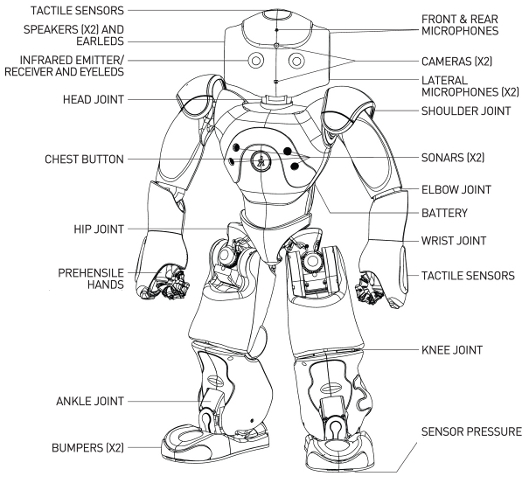
\includegraphics[width=0.75\linewidth]{Bilder/nao_h25_pres.png}
	\caption{Sensorenüberblick des NAO-H25 Version 6 \cite[in /H25]{nao_naoqi_docu}}
	\label{nao_v6_h25}
\end{figure}  

Das hier verwendete Modell ist NAO-H25 Version 6, dessen Sensoren in Abb. \ref{nao_v6_h25} zu sehen sind. Im Unterschied zu anderen Ausführungen besitzt NAO-H25 Drucksensoren an Händen und Fußsohlen. Er gehört zu den kommerziellen Robotern, deren Gelenke positionsbasierenden\hyphenation{posi-tions-basierenden} sind \cite{balance_strategy}, hat 25 Freiheitsgrade und wiegt $5,4\unit{kg}$. Über die an der Brust angebrachten Sonar Sensoren, die Kameras oberhalb und unterhalb der Augen Leuchtdioden, die vorder- und rückseitigen Mikrofone, den Stoßfängern an den Füßen sowie den Kontaktsensoren an Händen und Kopf kann der NAO mit seiner Umwelt vielseitig interagieren. Jedes Gelenk ist mit Sensoren für die Winkelmessung, den Stromverbrauch und die Temperaturmessung ausgerüstet. In seiner Brust befindet sich außerdem ein Gyroskop. Auf die in dieser Arbeit verwendeten Messausgaben wird im Folgenden genauer eingegangen.

\subsubsection*{Druckempfindlicher Widerstand}

An den Fußssohlen des NAO befinden sich pro Fuß vier sogenannte \textit{Force Sensitive Resistors} (FSR), zu sehen in Abb. \ref{hardware_semelles}. Diese ändern ihren Widerstand sobald Druck ausgeübt wird und messen im Bereich von 0 bis $25 \unit{N}$.

Die Ausgaben der Sensoren sind im Dateiverzeichnis des NAO hinterlegt und können jederzeit ausgelesen werden. Dies geschieht hier über dasselbe Pythonprogramm, welches ebenfalls die Bewegung steuert, näheres dazu in Kap. \ref{software} und im Anhang \ref{Anhang}.
Des Weiteren können der berechnete zweidimensionale Massenschwerpunkt und das Gesamtgewicht ausgegeben werden. Diese Werte sind allerdings unzuverlässig, sobald wenig oder kein Gewicht auf den Sensoren lastet. In \cite{pressure_shoe} haben Shayan et al. die eingebauten FSR mit barometrischen Drucksensoren verglichen und sind zu dem Schluss gekommen, dass die Sensoren, welche im NAO verbaut wurden, nicht sehr aussagekräftig sind. Deshalb werden hier die Ausgaben kritisch betrachtet, sowie die Balance des Roboters zusätzlich mit dem Gyroskop erfasst.
% Graph zu Gewicht des Naos (es wird weniger verzeichnet für MAP Sohlen)
\begin{figure}[tb]
	\centering
	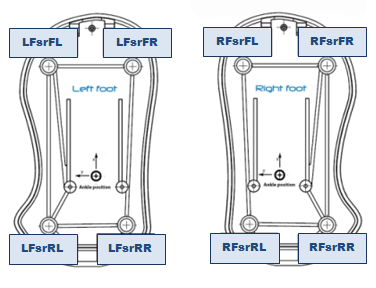
\includegraphics[width=0.6\linewidth]{Bilder/hardware_semelles.png}
	\caption{Drucksensoren und deren Bezeichnung in den Füßen von NAO \cite[ in /Technical overview/FSRs]{nao_docu_dev_guide}
	}
	\label{hardware_semelles}
\end{figure}

Eine weitere Einschränkung der Messungen ist die Kraftverteilung auf die FSRs. Dies hängt damit zusammen, dass ausschließlich Drucksensoren und die Zylinder für die Schrauben auf der Originalsohle anliegen. Dies ist für die Einlegesohlen aus Silikon bzw. MAP nicht der Fall, zu sehen in den Kapiteln \ref{Schuhkonstruktion} und folgende. Dies führt dazu, dass das Gewicht nicht mehr akkurat aufgenommen wird, siehe Abb. \ref{total_weight}. Hier wird deutlich, dass sich die Messung des Gewichtes etwa um $0,5 \unit{kg}$ von den NAO Schuhsohlen abweicht. 
% Graph zu Gewicht des Naos (es wird weniger verzeichnet für MAP Sohlen)
\begin{figure}[tb]
	\centering
	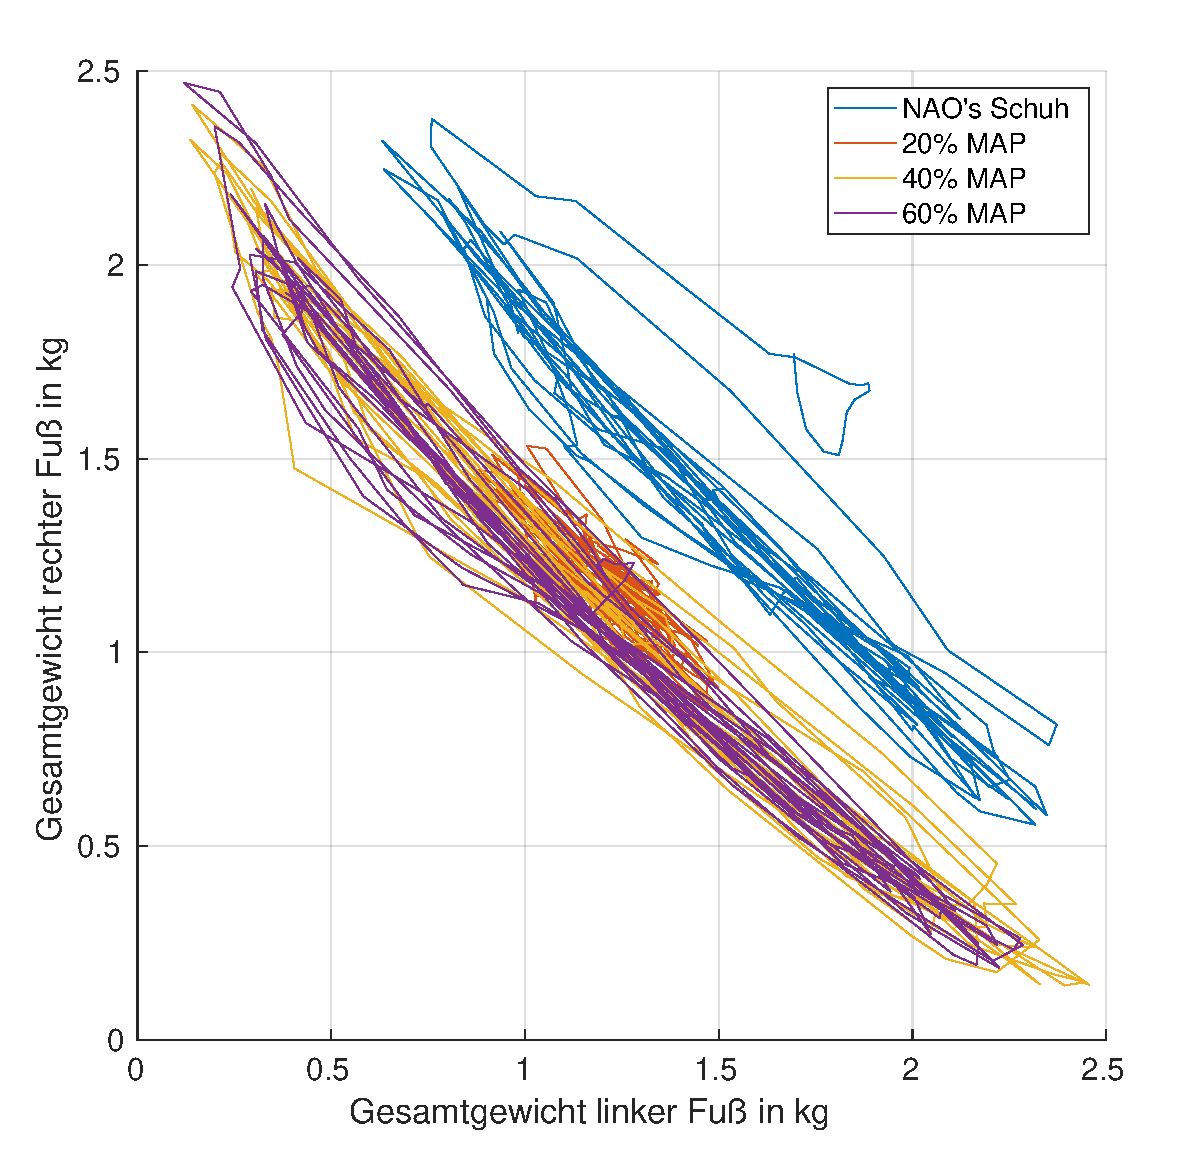
\includegraphics[width=0.8\linewidth]{Bilder/TotalWeight_Grund_20_40_60_mean.pdf}
	\caption{Berechnetes Gesamtgewicht der Messungen für die normalen Sohlen von NAO in blau und dem Silikon versetzt mit Eisenpartikeln in 20\%, 40\% und 60\% Anteilen. Das Gewicht wird in $\unit{kg}$ ausgegeben.}
	\label{total_weight}
\end{figure}

\subsubsection*{Aktoren und Sensoren der Beinen}
Neben den bereits beschrieben Drucksensoren hat NAO eine Ausgabe für jeden eingebauten Aktor mit den Werten:
\begin{itemize}
	\item ...\texttt{/Position/Actuator/Value} (\texttt{Pos/Act})
	\item ...\texttt{/Position/Sensor/Value} (\texttt{Pos/Sens})
	\item ...\texttt{/ElectricCurrent/Sensor/Value} (\texttt{Current})
	\item ...\texttt{/Temperature/Sensor/Value}
	\item ...\texttt{/Hardness/Actuator/Value} 
	\item ...\texttt{/Temperature/Sensor/Status} 
\end{itemize}
Hierbei unterscheiden sich die Pfade bei \glqq ...\grqq{} je nach Aktor. Die Bezeichnungen in Klammern dahinter dienen der abkürzenden Benennung für spätere Kapitel. Der Effekt der Sohlen auf die Aktoren wurde mit \texttt{AnkleRoll} und \texttt{AnklePitch} zu sehen in Abb. \ref{hardware_legjoint} aufgenommen.

\begin{figure}[b!]
	\hfill
	\begin{subfigure}[c]{\linewidth}
		\centering
		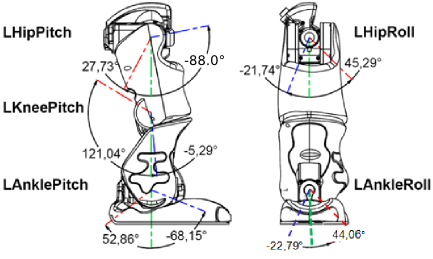
\includegraphics[width=0.7\linewidth]{Bilder/hardware_llegjoint.png}
	\end{subfigure}
	\begin{subfigure}[c]{\linewidth}
		\centering
		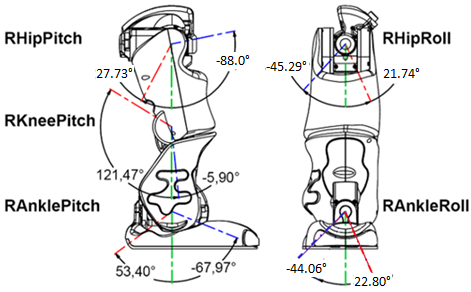
\includegraphics[width=0.7\linewidth]{Bilder/hardware_rlegjoint.png}
	\end{subfigure}
	\hfill
	\caption{Das obere Bild zeigt Vorder- und Seitenansicht der Positionen und möglichen Winkel des linken Beins. Die untere Abbildung veranschaulicht dieselben Parameter für das rechte Bein. \cite[in /kinematics-data/joints]{nao_docu_dev_guide}}
	\label{hardware_legjoint}
	%\vspace{0.1cm}
\end{figure}

Die Temperaturausgaben sowie die Starrheit der Motoren liefern keine verwertbaren Messausgaben, da sich beide während einer Messung nicht oder kaum ändern. \texttt{Pos/Act} und \texttt{Pos/Sens} geben ähnliche Werte in $\unit{rad}$ aus, da ersteres die Ausgabe des Programms vorgibt und zweiteres den tatsächlich gemessenen Wert an dem Gelenk ausgibt. Der \texttt{Current} Wert wird in Ampère gemessen und gibt an, wie viel Strom für das Erreichen der entsprechenden Aktorposition und Starrheit aufgewendet werden muss. Dies bedeutet, dass dieser Wert unter anderem eine Aussage über den Zustand des Aktors geben kann. 

Bei den Probegängen des NAO stellte sich heraus, dass er in einer Kurve nach links läuft bei einem Befehl, der ihn hätte gerade aus laufen lassen sollen. Softbank Robotics betonte, dass es nicht möglich ist, dass NAO komplett gerade läuft. Grund dafür ist zum einen, dass die Motoren nicht immer komplett identisch hergestellt sind. Zum anderen ist der Gehbefehl, welcher hier ausgeführt wird, ohne Rückkopplungsschleife für Einwirkungen der Umgebung ausgestattet. Näheres zur Software wird in Kapitel \ref{software} beschrieben.

% Jetzt kommt der Testgang und alle Graphen, die damit zusammenhängen.

% Aktoren und Sensoren in den Beinen
% Ausgabe eines Sensors und technische Details
% Wichtige Ausgaben für Stabilität
% fehlerhafter Gang

\subsubsection*{Gyroskop}
Der NAO Roboter verfügt über eine Inertialeinheit, welche sich zusammensetzt aus den 3 Achsen des Gyrometers, im einer Achsengeschwindigkeit von bis zu $500^\circ\unit{/s}$, sowie den 3 Achsen des Beschleunigungssensors, mit einer Beschleunigung bis zu $2\unit{g}$ \cite[/Technical overview/Inertial unit]{nao_docu_dev_guide}. Die Z-Achse des Gyroskops, welche die Höhenorientierung des Roboters ausgeben würde, ist allerdings noch nicht verfügbar. Außerdem wird durch diese beiden Sensoren der Winkel des Torsos bestimmt. 
\FloatBarrier

\subsection{Verwendete Software} \label{software}
\subsubsection*{Die Rahmenumgebung NAOqi}
NAOqi wird die Hauptsoftware genannt, welche auf diesem Roboter sowie auf Pepper läuft, das Betriebssystem NAOqi OS basiert auf Linux. Der NAOqi Rahmen ist eine plattformübergreifende und sprachenübergreifende Umgebung, mithilfe derer Anwendungen für den NAO erstellt werden können. Sie kann über Windows, MacOS und Linux verwendet werden und es werden die Sprachen Python und \texttt{C++} unterstützt, wobei ersteres direkt auf dem NAO kompiliert werden kann, während \texttt{C++} komplizierter benutzt wird, aber mehr Eingriffe erlaubt. \cite[/Former NAOqi Framework/Key concepts]{naoqi_dev_guide}

Außerdem gibt es eine Desktop Anwendung namens Choregraphe in der Dialoge und Verhaltensmuster erstellt werden können ohne Code schreiben zu müssen. Hierüber ist der Akkustand und aktuelle Position in Form eines virtuellen Bildes des tatsächlichen NAO einsehbar, sowie der autonome Zustand ein- und ausschaltbar. \cite[/Choregraphe Suite/What is Choregraphe]{naoqi_dev_guide}

Für die in dieser Masterarbeit benötigten Anwendungen war Python am besten geeignet. Erforderlich waren eine sich wiederholende Schrittabfolge sowie die Aufzeichnung diverser bereits im NAO verbauten Sensoren. Text verarbeitende Funktionen sind in dieser Sprache leicht zu erhalten und anzupassen. Es wurde sich für den \texttt{moveTo()} Befehl als Fortbewegungsmethode entschieden, denn dieser wird durch das Objekt \texttt{post} zu einem sogenannten \textit{non-blocking call}. Dies ermöglicht das Aufrufen von weiteren Befehlen zeitgleich zur Bewegung. Der Nachteil ist, dass der Gang dadurch unbeaufsichtigt vonstatten geht, d.h. NAO kann seine Schritte nicht seiner Umgebung anpassen. Die aufgezeichneten Daten werden in eine csv Datei übertragen und mit Matlab ausgewertet. Im Anhang ist der gesamte Programmcode \ref{Messungscode} abgebildet, welcher auf dem NAO ausgeführt wird. 

\subsubsection*{Konstruktionssoftware}	
Das CAD-Programm Inventor von Autodesk ist für 3D Konstruktionen ausgelegt und bietet einige nützliche Simulationserweiterungen, welche unter anderem einen Shape Generator enthält \cite{inventor}. Dieser kann Flächen minimieren während die Stabilität erhalten bleibt, sodass ein minimaler Anteil an Material verwendet wird \cite{shape_generator}. 

Für die Herstellung der Prototypen und Gussformen wurde das FDM (fused deposition modeling) 3D Druckverfahren mit PLA oder PETG Filamenten von filamentworld \cite{filament} verwendet und für die Vorbereitung auf den Druck der Slicer Cura von Ultimaker \cite{cura}.

\subsubsection*{Datenauswertung mit Matlab}
Für die Auswertung wurden neben der gewöhnlichen \texttt{plot} Funktion von Matlab \cite{matlab} auch die \textit{Statistics and Maschine Learning} Toolbox mit deskriptiver Statistik und Visualisierung verwendet \cite{toolbox}. 
Eine Messreihe ergibt sich aus 40 Messungswiederholungen, in denen NAO etwa einen Meter zurücklegt. Jede Auswertung enthält das arithmetische Mittel eines Sensors von allen Messungen der Messreihe. Diese Mittel wurden mit dem Befehl \texttt{mean()} berechnet und mit Werten aus weiteren Messreihen, mit anderem Schuh oder anderen Untergrundvoraussetzungen aber gleicher Schrittlänge und Sensorenmessung verglichen. Dieser Vergleich wurde mit den Funktionen \texttt{hist} und \texttt{scatterhist} der genannten Toolbox angestellt. Ersteres erstellt ein Histogramm und ist damit optimal für eine Häufigkeitsverteilung. Zweiteres erstellt einen aus zwei Vektoren resultierenden Scatterplot sowie zwei Histogramme, welche die Häufigkeitsverteilung der jeweiligen Vektoren darstellen. Dies ermöglicht eine umfangreiche Verteilungsanalyse für Sensorausgaben, die sich aus zwei Achsen zusammensetzen, wie z.B. der 2 dimensionalen Gyroskop Ausgabe.

Das arithmetische Mittel berechnet Matlab durch \cite[S.50]{statistik_Ludwig}
\begin{equation} \label{mean}
	\bar{x} = \frac{1}{n} (x_1 + x_2 + \dots + x_n) = \frac{1}{n}\sum_{i=1}^{n}x_i
\end{equation}
und wurde auf eine Messreihe angewendet. Die Darstellung der Verteilungen per Histogramm wurde ergänzt durch ein gleitendes Histogramm, errechnet durch den Kern-Dichteschätzer \cite[S.93]{statistik_Ludwig}
\begin{align} \label{pdf}
	\hat{f}(x)=\frac{1}{nh} \sum_{i=1}^{n}K\left(\frac{x - x_i}{h}\right),\, x \in \mathds{R}
\end{align}
mit dem Gauss-Kern \cite[S.93]{statistik_Ludwig}, 
\begin{align}
	K(u) = \frac{1}{\sqrt{2\pi}} \exp\left(-\frac{1}{2}u^2\right),\, u \in \mathds{R}
\end{align}
welcher in Matlab mit \texttt{'Kernel'} und dann standardmäßig mit \texttt{'normal'} in der \texttt{fitdist()} Funktion aufgerufen wird \cite{kernel-distribution} \cite{fitdist}. Das Scatterhistogramm ermöglicht dieselbe Verwendung dieser Distribution. Bei den in dieser Arbeit verwendeten Graphen ist zu beachten, dass die jeweilige x bzw. y Kompontente mit einer Häufigkeitsskala ausgestattet ist, welche sich auf das Histogramm bezieht. Das bedeutet, die Häufigkeit, welche auf der jeweiligen y-Achse der Wahrscheinlichkeitsdichten neben den Scatterplots angezeigt wird, hängt von den Histrogrammbalkenbreite, d.h. von der Breite der x-Achse ab, die wiederum von der Breite des Scatterplots abhängt.  

Schließlich wurde für eine Veranschaulichung der Verteilung der Dichtefunktionen die Halbwertsbreiten für das Gyroskop, den Beschleunigungssensor und die Winkelangabe berechnet mit:
\begin{align}
	|x_1 - x_2|&, & \text{für } f(x_1)&=f(x_2)=\frac{1}{2}f(x_\text{max}).
\end{align}


\FloatBarrier

\subsection{Magneto-aktive Polymere}\label{kap_MAP}
%	 woher kommt der begriff, was ist es
%	 woher bestand die bisherige Forschung, warum ist es interessant
Der Begriff Magneto-Aktive Polymere (MAP) gehört zur Gruppe der intelligenten, auf magnetische Felder ansprechende Materialien, welche typischerweise Kombinationen aus einer weichen Polymermatrix und darin eingebetteten, magnetischen Partikeln sind. Diese Partikel werden während dem Vernetzungsprozess des Polymers in dieses eingebettet. 

Die wesentlichen Verhaltensweisen, die MAP in der heutigen Zeit attraktiv für seine Verwendung macht, wurde bereits in den 80ger Jahren von Rigbi und Jilken \cite{Rigbi1} sowie Rigbi und Mark \cite{Rigbi2} beschrieben. Ein Jahrzehnt später wurde eine genauere Analyse zum ersten Mal von Ginder und Jolly et al. \cite{ginder} veröffentlicht. 
Diese aus mehreren Komponenten bestehenden Materialien stechen durch zwei Schlüsseleigenschaften heraus. 
Zum einen das magnetostriktive Verhalten, bei dem es sich um das Phänomen der Verformung eines Materials handelt, welches durch ein Magnetfeld hervorgerufen wird \cite{Martin_2006}.
Zum anderen die veränderbaren Materialeigenschaften wie Elastizität und Dämpfungsfaktor, welche hauptsächlich mit der Mikrostruktur des Grundlagenmaterials zusammenhängen. \cite{Varga1} \cite{Varga2}

Außerdem ist entscheidend, wie die magnetischen Partikel in das Polymer eingebettet werden. Je nachdem ob während des Vernetzungsprozesses ein Magnetfeld wirkt, können sich die Partikel kettenförmig ausrichten und dadurch dem MAP eine anisotropisches Verhalten zuführen. Isotropisches MAP hingegen enthält keine gerichteten Partikel. Diese verschiedenen Ausrichtungsarten und Herstellungsarten können sowohl die Steifigkeit verändern, als auch bestimmen, ob das MAP in einem Magnetfeld ausgedehnt oder zusammengedrückt wird. 

Weiche, mit einem Feld manipulierbare, Polymere haben diverse Anwendungsbereiche in akademischen und industriellen Bereichen. Angefangen von anpassungsfähiger Vibrationsabsorption in der Luftfahrt und Automobilindustrie durch das Einsetzen durch Scherung \cite{Ginder_Schlotter_Nichols} \cite{Deng_Gong}, Windung \cite{Hoang_Zhang_Li_Du} und Kompression bzw. Elongation \cite{Kallio_2007} und Vibrationsisolatoren \cite{Ginder_2000} sowie Sensoren \cite{Ginder_2000} \cite{Martin_2006}, Ventile und Aktoren \cite{Boese_2012} \cite{Keip_2014} und anpassungsfähige, sandwichartige Strukturen \cite{Zhou_2005} \cite{Zhou_2006} \cite{Wei_2008} bis hin zur Anwendung in der Bionik wie zum Beispiel durch Mikro- und Nanoroboter und Schwimmroboter \cite{Qiu_2015} \cite{Xu_2015} \cite{Lum_2016} \cite{Hu_2018}, Schlauchradpumpen \cite{Fuhrer_2013} und Erschütterungsdämpfer \cite{Li_2013}.

Des Weiteren wird die Verhärtung bei Anlegen eines Magnetfeldes für Greifer genutzt \cite{Qi_2020}, ebenso wird der 3D Druck von magneto-aktiven Polymeren \cite{Sindersberger_2018} bereits erforscht.

%\subsection{Magnetostiction}
%
%Der Begriff Stiction ist in erster Linie eine englische Wortneuschöpfung aus dem Wort \textit{friction}, also Reibungskraft und \textit{sticking}, also kleben. Ersteres wird unterschieden in Haftreibung, welche den Schwellenwert einer äußeren Kraft darstellt, der überwunden werden muss um ein Objekt in Bewegung zu versetzen, sowie in Gleitreibung, welche den Widerstand, der entgegen der Bewegungsrichtung wirkt, beschreibt. Stiction entsteht wenn die Haftreibung die Gleitreibung übersteigt. Dies sorgt für einen plötzlichen Stillstand, bis dann die auf das Objekt wirkende Kraft ausreicht, um eine erneute Bewegung zu erlauben. Dies kann zu ruckartigen Bewegungen führen und ist deshalb in vielen Fällen eine unerwünschte Eigenschaft \cite{Ruel2014STICTIONT}. Es gilt dies nicht zu verwechseln mit Adhäsion, welche entsteht, wenn z.B. Silikon auf dem Boden flach aufliegt und sich an den Boden auf die Art anpasst, dass bei dem Versuch, es zu schieben, sich an den Boden anklebt. Wenn die Adhäsion fehlt, aber die Reibung noch kontrollierbar ist, dann handelt es sich um Stiction. \cite{Monkman_2019}

\subsection{Carbonyleisenpulver} \label{cip}

\begin{wrapfigure}{hr}{0.5\linewidth}
	%\vspace{-0.5cm}
	\centering
	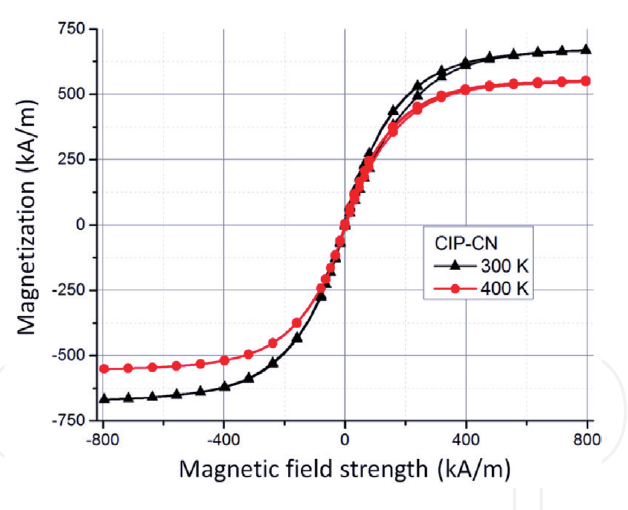
\includegraphics[width=\linewidth]{Bilder/Hysterese.png}
	\caption{Hysteresekurve von CIP entnommen aus \cite[Abb.4]{Magnetorheological_Elastomers}}
	\label{Hysterese}
	\vspace{-0.6cm}
\end{wrapfigure}
% magnetische Eigenschaften -> suszeptibiltiät
% Was sagt suszeptibilität aus? Was bedeutet das für das Carbonyleisenpulver
Bei den in dieser Arbeit verwendeten magnetischen Partikel für die Herstellung des MAP handelt es sich um das von BASF vor über 85 Jahren entdeckte Carbonyleisenpulver (engl. \textit{carbonyl iron powder)}, CIP) \cite{basf_cip_allg}. 
Es wird durch thermische Zersetzung von Eisenpentacarbonyl hergestellt und besteht aus Teilchen in einer Größenordnung von 5 bis $1 \unit{\mu m}$.

% bin mir nicht sicher, ob hier noch mehr hin muss

Die magnetischen Eigenschaften dieses Materials lassen sich durch die Suszeptibilität \cite[Gleichung (2)]{Gorodkin}
\begin{equation}
	\chi = \frac{3 \chi_p}{3 + \chi_p} \,\phi
\end{equation}
mit $\chi_p$ als Suszeptibilität der einzelnen Teilchen und einem Partikel Volumen $\phi$ welches sehr viel kleiner als 1 ist, beschreiben. 
CIP zählt zu den ferromagnetisch weichen Materialien, was sich durch Untersuchungen der Hysteresekurve veranschaulichen lässt, wie zum Beispiel von Liu u.a. \cite{Magnetorheological_Elastomers} zu sehen in Abb. \ref{Hysterese}






%%% Local Variables:
%%% mode: latex
%%% TeX-master: "main"
%%% End:
% MAP
% Nao
% Software: Matlab, Autodesk Inventors, Naos Software
% Ziel der Arbeit
\newpage
\section{Versuchsaufbau}
In diesem Kapitel wird auf alle selbstkonstruierten Komponenten eingegangen, welche für die Messungen benötigt wurden. Zum einen gibt es eine Schuhkonstruktion, die es erlaubt, die in einer Gussform angefertigten MAP Sohlen einzuhängen, zum anderen wurde ein Laufsteg mit Rampenfunktion entworfen, welcher es erlaubt, Magnete unter die Lauffläche zu montieren. 

\subsection{Schuhkonstruktion} \label{Schuhkonstruktion}
\begin{figure}[tb]
	\hfill
	%\centering
	\begin{subfigure}[c]{.49\linewidth}
		\centering
		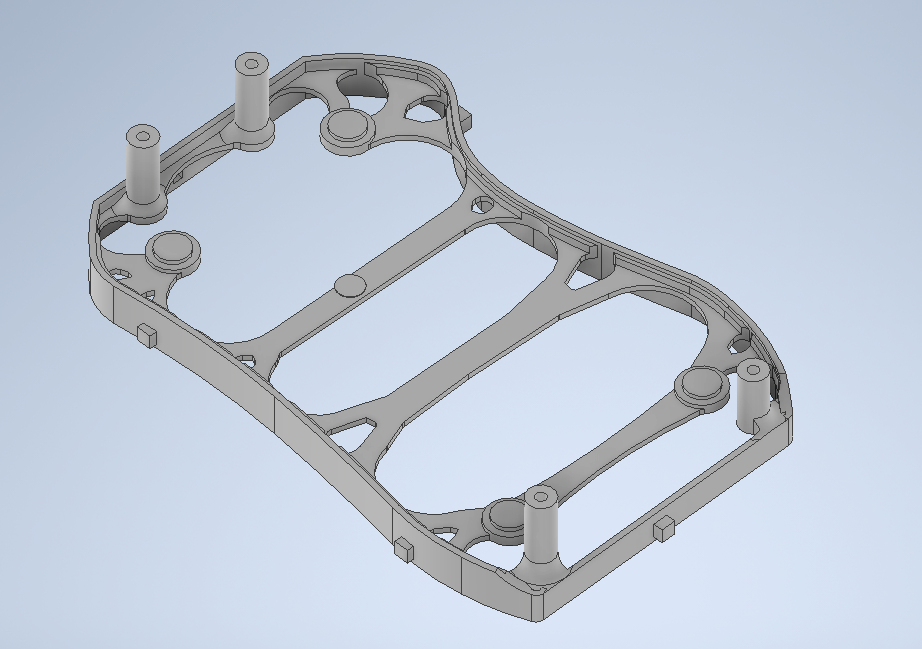
\includegraphics[width=\linewidth]{Bilder/Schuh_oben.png}
	\end{subfigure}
	\begin{subfigure}[c]{.49\linewidth}
		\centering
		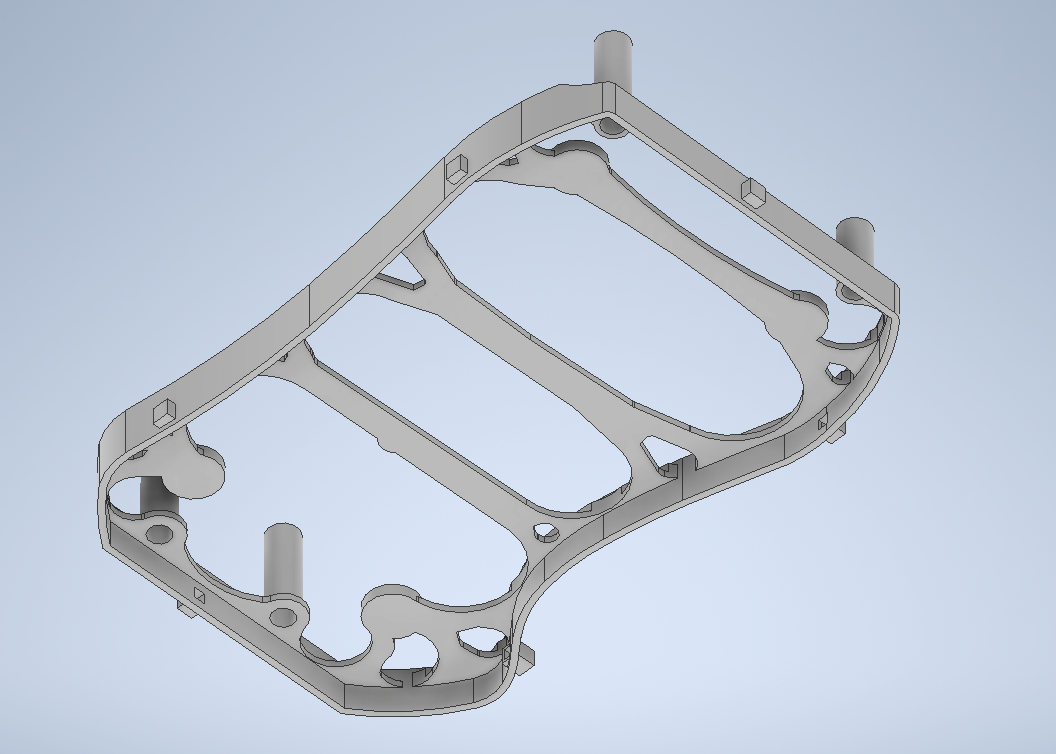
\includegraphics[width=\linewidth]{Bilder/Schuh_unten.png}
	\end{subfigure}
	\hfill
	\caption{Linker Schuh in Autodesk Inventors, Links von Oben, Rechts von Unten.}
	\label{Schuh_Inventor}
	%\vspace{0.1cm}
\end{figure}
Die Hülle eines Fußes von NAO besteht aus einem zweiteiligen Oberteil, welches das Fußgelenk abschließt und einem unteren Teil, welcher mit 4 Schrauben angebracht wird. Ohne Schraubenbefestigung liegt der Fuß nicht fest an. Die in Kapitel \ref{aufbau_NAO} beschriebenen vier Drucksensoren liegen dabei in dem unteren Teil auf Erhöhungen auf. Um die Auswirkungen anderer Sohlen für NAO messen zu können, muss der untere Teil des Fußes ausgetauscht werden. Dieser 	\glqq Schuh\grqq{} welcher die ursprüngliche Fußsohle ersetzt, enthält wiederum einen Steckplatz für die MAP Sohlen in verschiedenen Stärkegraden. 

In Abb. \ref{Schuh_Inventor} sind links die vier flachen Zylinder zu sehen, auf denen die Drucksensoren aufliegen. Die vier Zylinder an den Seiten sind die Führung der Schrauben, welche an das obere Teil des Fußes von NAO geschraubt werden. Die Außenform umschließt den oberen Teil während eine zweite Erhöhung, welche an den Innenseiten verläuft, auf dem Rand des oberen Teils aufsitzt, sodass die Passform fest ineinander greift. Da das gesamte Gewicht des NAO auf den 4 Drucksensoren lastet, kann Druckmaterial für die restliche Gesamtfläche bis auf stabilitätserhaltende Streben eingespaart werden. Diese Form wurde mit dem Shape Generator von Autodesk Inventor generiert, sodass sie längs bis zu einem $45^\circ$ Winkel ohne zu brechen gebogen werden kann. Die instabilsten Stellen sind die Zylinder der Schraubvorrichtung, welche durch Fillets verstärkt wurden. Diese Instabilität ist auf den schichtweise Druckvorgang durch das FDM Verfahren geschuldet und kann durch kleinere Schichthöhen ausgeglichen werden.

Die Unterseite, zu sehen in Abb. \ref{Schuh_Inventor} rechts, ist ein Hohlraum für die MAP Sohle zusammen mit den viereckigen Steckeinlässen für die Halterung. Die Seiten des Schuhs sind so hoch, dass das MAP etwa $1 \unit{mm}$ herausragt. Andernfalls würde NAO auf der Schuhkante laufen und nicht auf dem MAP.  
% wesentliche Aufgabe des Schuhs
% Stabiler Ersatz der vorherigen Sohle -> hält nur mit den Schrauben
% Druckverteilung auf die Sensoren 
% Einsparung von Material in der Mitte
% Anpassung an den oberen Teil durch Auflage und Umfassung
% Einfassung des MAPs
% Basiert auf dem Scan des zweiteiligen Fußes von NAO.
% 4 Schrauben befestigen den unteren Teil an das obere Teil. Der Schuh ersetzt die eigentliche Sohle
% Das Gewicht des Roboters lastet hauptsächlich auf den 4 Drucksensoren, welche in Kap (Theorie) bereits erklärt wurden. Die 4 kreisförmigen Flächen liegen deshalb genau da an, wo diese Sensoren auch in dem ursprünglichen Teil anlagen. 
% Shape generater tragende Oberfläche.

\subsection{Herstellung des MAP} \FloatBarrier
Der Herstellungsprozess allein dauert nicht mehr als eine halbe Stunde. Zunächst muss das Verhältnis für den Anteil des CIPs bestimmt werden. Die Masse ergibt sich aus
\begin{equation}
\text{m}_{\text{CIP}} = \frac{Ratio_{\text{CIP}} [\%]}{100\%}\cdot\text{m}_{ges},
\end{equation}
Die beiden additiven Komponenten A und B, welche auch als Basis und Katalysator bezeichnet werden, sind im Verhältnis 1:1 zu mischen. Das Volumen in \unit{ml} ergibt sich aus:
\begin{align}
\text{V}_\text{A} &= \frac{\text{m}_\text{A}}{\rho_\text{A}} ,& 
\text{V}_\text{B} &= \frac{\text{m}_\text{B}}{\rho_\text{B}}
\end{align}
mit $\rho_\text{A} = 1.071$ sowie $\rho_\text{B} = 1.046$ sowie
\begin{align}	
\text{m}_\text{A} &= \left( 1- \frac{Ratio_{\text{CIP}} [\%]}{100\%}\right)\times
\frac{\text{m}_{ges}}{\alpha + \beta}\times\alpha ,&
\text{m}_\text{B} &= \left( 1- \frac{Ratio_{\text{CIP}} [\%]}{100\%}\right)\times
\frac{\text{m}_{ges}}{\alpha + \beta}\times\beta,
\end{align}
Die Platzhalter $\alpha$ und $\beta$ stehen für das Mischverhältnis der jeweiligen Komponenten und sind hier Beide gleich 1, sodass die Formeln vereinfacht werden können in:
\begin{align}	
\text{m}_\text{A} &= \left( 1- \frac{Ratio_{\text{CIP}} [\%]}{100\%}\right)\times
\frac{\text{m}_{ges}}{2} ,&
\text{m}_\text{B} &= \left( 1- \frac{Ratio_{\text{CIP}} [\%]}{100\%}\right)\times
\frac{\text{m}_{ges}}{2}.
\end{align}

\begin{figure}[b]
	\hfill
	%\centering
	\begin{subfigure}[c]{.49\linewidth}
		\centering
		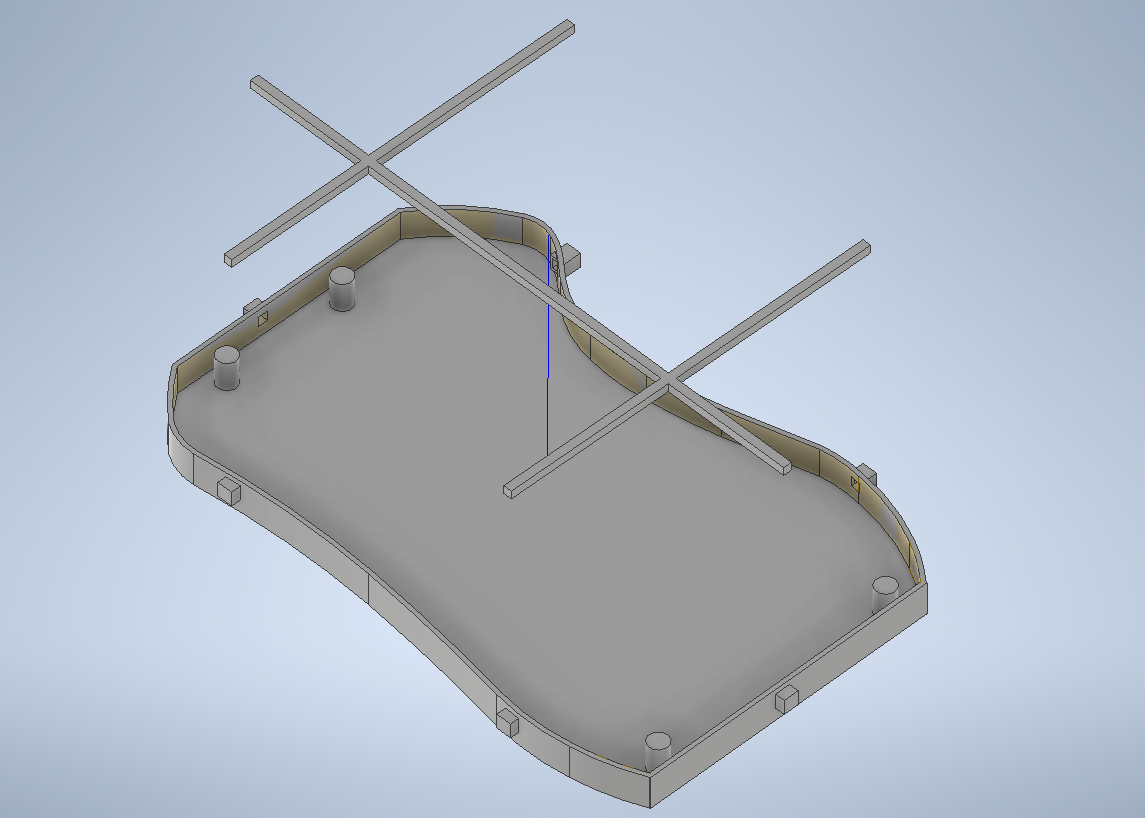
\includegraphics[width=\linewidth]{Bilder/Gussform_Innenteil_verschoben.png}
	\end{subfigure}
	\begin{subfigure}[c]{.49\linewidth}
		\centering
		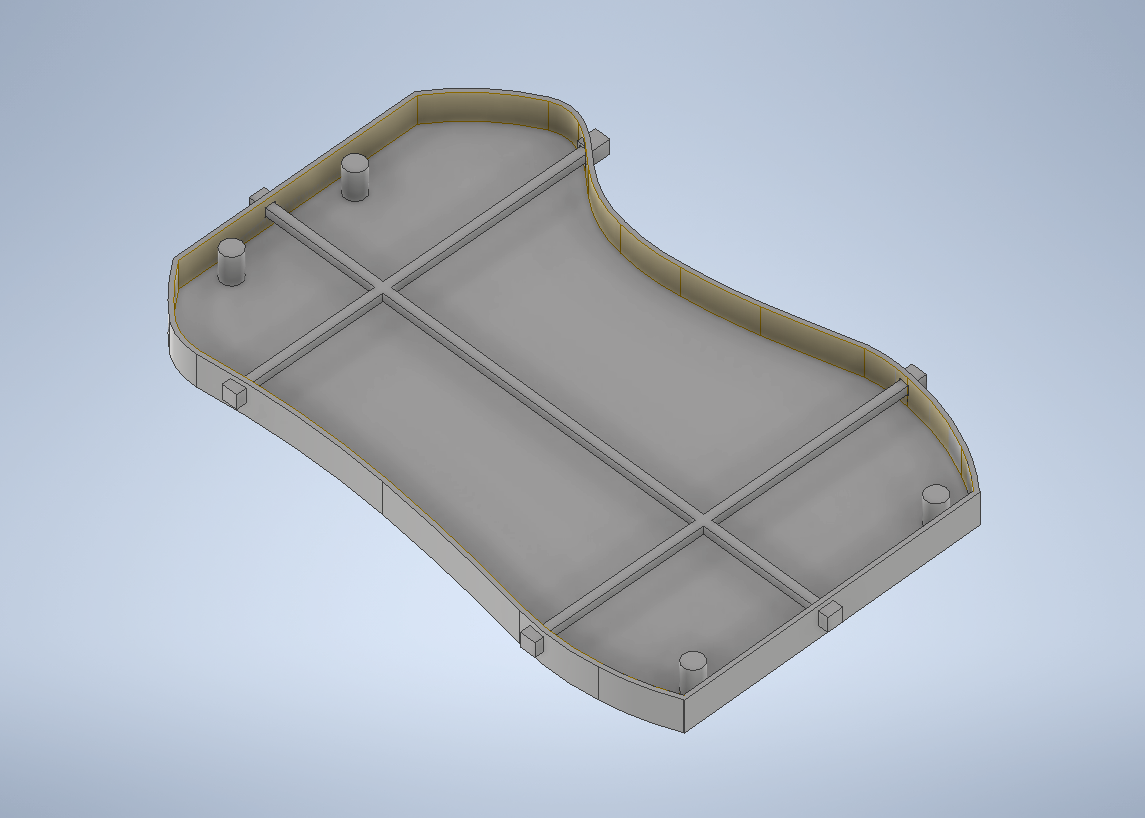
\includegraphics[width=\linewidth]{Bilder/Gussform.png}		
	\end{subfigure}
	\hfill
	\caption{Gussform der MAP Sohlen. Links ist die Innenhalterung herausgenommen, rechts ist sie eingespannt in den sechs Eckhalterungen.}
	\label{Gussform_Inventor}
	%\vspace{0.1cm}
\end{figure}

Mit der Laborwaage ABT 120-5DM von Kern wird $\text{m}_\text{CIP}$ in einem Becher abgemessen. Mit den Spritzen lassen sich $\text{V}_\text{A}$ und $\text{V}_\text{B}$ auf die ersten Nachkommastelle genau beifügen. Es handelt sich um SF13 2k-Silikon vom Hersteller Silikon Fabrik. Der Becherinhalt wird dann mit einem kleinen Mixstab gemischt, um eine gleichmäßige Verteilung der beiden Komponenten zu erreichen und somit eine optimale Vernetzung zu gewährleisten. Anschließend wird die Probe in einen Exsikkator gestellt, welcher mit einer Vakuumpumpe entgast wird, sodass das Silikon entgast ist. Schließlich kann das bis dahin noch flüssige MAP in die Gussform gegossen werden, nach spätestens einem Tag ist die Sohle dann komplett vernetzt. 

Da Silikon selbst sich nur sehr schlecht durch etwaige Klebstoffe nach der Vernetzung verkleben lässt wird hier wie in Abb. \ref{Gussform_Inventor} zu sehen ist, eine $2\unit{mm}$ dicke Stangenkonstruktion eingehängt, welche bis auf die 6 Enden mit MAP umschlossen wird. Dieses aus PLA gedruckte Konstrukt ist flexibel und kann deshalb durch Verbiegen in die Verankerungen gedrückt werden. Nach der vollständigen Vernetzung kann die Sohle aus der Form entnommen und in den Schuh aus dem vorherigen Kapitel eingesetzt werden. 

Die vier Zylinder dienen als Platzhalter um die sechs Ecken in der Halterung des Schuhs für einen besseren Halt festzukleben und dann durch die Löcher des MAPs die Schrauben lockern zu können. 

Das Silikon selbst hat eine zu große Haftung, v.a. durch die Fläche des Schuhs. Deshalb wird es vor der Messung mit Speisestärke eingedeckt, was eine Bodenhaftung ähnlich der Plastiksohle des Originalschuhs von NAO zur Folge hat. Dies verhindert außerdem ungewollte Adhäsion.

\subsection{Laufstegkonstruktion} \FloatBarrier

Der NAO Roboter ist für den Einsatz auf geraden Bodenflächen im Innenbereich ausgelegt wobei er bei einem Bewegungsablauf ohne Anpassung an die Umwelt wie mit dem Befehl \texttt{moveTo()} durch Rutschen nicht immer die gleiche Strecke zurücklegt. 
Um wiederholbare Messreihen garantieren zu können ist eine Teststrecke von Nöten. Des Weiteren sind verschiedene, flache Untergründe für eine Sohlenentwicklung interessant.
\begin{figure}[hb]
	\hfill
	%\centering
	\begin{subfigure}[c]{.49\linewidth}
		\centering
		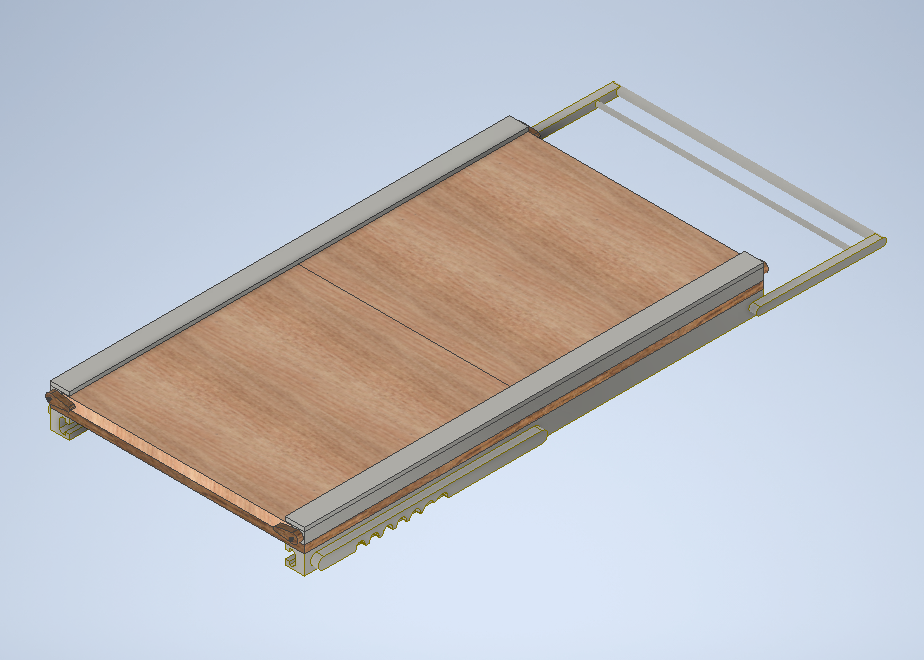
\includegraphics[width=\linewidth]{Bilder/Rampe_oben.png}
	\end{subfigure}
	\begin{subfigure}[c]{.49\linewidth}
		\centering
		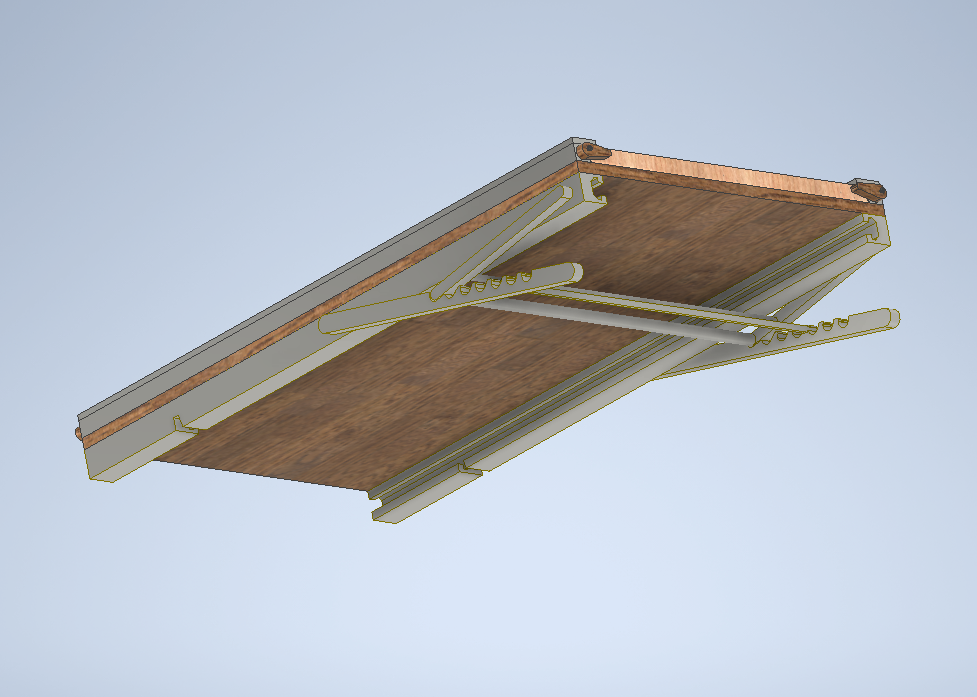
\includegraphics[width=\linewidth]{Bilder/Rampe_unten.png}
	\end{subfigure}
	\hfill
	\caption{Laufstegrampenkonstruktion mit zwei austauschbaren Platten und einer Winkelverstellung mit Raste. Links: Sicht von schräg oben mit eingeklappter Winkelverstellung. Rechts: Sicht von schräg unten mit niedigster Winkeleinstellung.}
	\label{Rampe_Inventor}
	%\vspace{0.1cm}
\end{figure}
Außerdem kann auf das MAP nur Einfluss genommen werden, wenn ein magnetisches Feld angelegt wird. Deshalb wurde ein Laufsteg mit einem Hohlraum angefertigt, um unter der Fläche, auf der NAO läuft, Magneten anzubringen. 

\begin{wrapfigure}{hr}{0.4\linewidth}
	\vspace{-0.5cm}
	\centering
	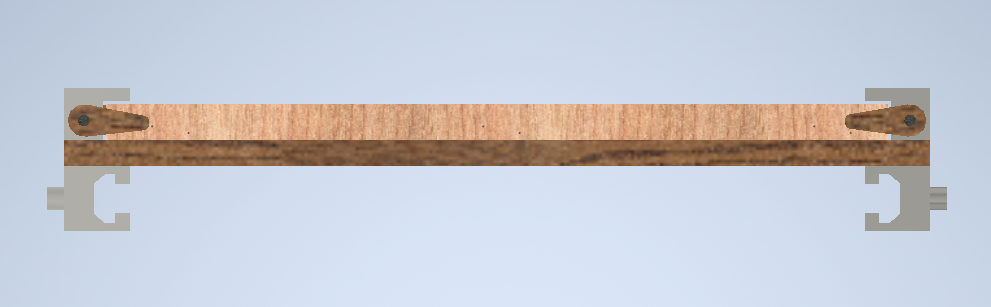
\includegraphics[width=\linewidth]{Bilder/Rampe_Seitenansicht3.png}
	\caption{Seitenansicht der Rampe mit einer Breite von $66,4 \unit{cm}$.}
	\label{Rampe_Seite_Inventor}
	\vspace{-0.5cm}
\end{wrapfigure}

% Aufbau der Rampe
Der Laufsteg besteht aus einer $120\times66,4 \unit{cm}$ großen Pressholzplatte, die auf der Oberseite mit einem Aluminiumkonstrukt erweitert ist, welches die Einschubplatten von beiden Längsseiten und nach oben hin abschließt, Abb. \ref{Rampe_Inventor} links. Auf den kurzen Seiten verriegeln jeweils zwei drehbare Keile den Einschub, sodass die Platten eingeschlossen werden, Abb. \ref{Rampe_Seite_Inventor}.

Auf der Unterseite sind an den Längsseiten zwei mit T-Nut versehene Aluminiumstangen angebracht, sowie eine zweiteilige Stangenkonstruktion, die eine Winkelverstellung mit Raste erlaubt, zu sehen in Abb. \ref{Rampe_Inventor} rechts. Die einstellbaren Winkel betragen ca. $5^\circ$ bis $17^\circ$, oder es wird für $0^\circ$ vollständig eingeklappt.
  
Man hat NAO bereits schräge Flächen gehen lassen wie in \cite{Lutz_naowalking}. Dies erfordert einen komplett anderen Gang und wäre über den zeitlichen Rahmen dieser Arbeit hinausgegangen. Die Neodymmagnete, die verwendet wurden, haben eine Haftkraft von ca. $16 \unit{kg}$, eine Maße von $40\times40\times4 \unit{mm}$ \cite{schraubmagnet} und wurden an die Unterseite der Rampe geschraubt. Die ersten Versuche ergaben schließlich, dass das MAP nur bei einem Abstand ohne Einlageplatten reagierte. Deshalb wurden in den gesamten Messungen ohne diese Platten durchgeführt. 

\FloatBarrier
% Was man für die Messungen verwendet hat

%\subsubsection{Genaueres zum Einsatz an dem Nao Roboter}

%%% Local Variables:
%%% mode: latex
%%% TeX-master: "main"
%%% End:
% Schuh
% MAP Herstellung und Anbringung
% Rampe
%
\newpage
\section{Versuchsdurchführung}
Bereits in den vorherigen Kapiteln wurde auf die Durchführung dieses Versuchs eingegangen. Im folgenden wird über den Ablauf und einige Problematiken gesprochen, welche sich während dem Herstellungs- und Laufprozess herauskristallisierten. 

Wie bereits in Kapitel \ref{Herstellung_MAP} beschrieben, wird zunächst das MAP hergestellt und anschließend in die Formen gegossen. Während der Vermengung wurde festgestellt, dass bei 60\,\%gem MAP die Durchmischung nicht gewährleistet werden kann, solang der verwendete Becher über die Hälfte voll ist. Deshalb wurden in diesem Fall zwei identische Proben hergestellt, welche erst in der Form zusammengegossen wurden. Alle anderen Proben mussten nach der Durchmischung in zwei separate Becher umverteilt werden, da während der Entgasung das Gemisch an Volumen bis zu einer Druckabnahme von etwa $15 \unit{mbar}$ zunimmt. Dies hat zur Folge, dass der Becher nur etwa halb voll sein darf, damit das MAP nicht \glqq überkocht\grqq{}. 

Nach spätestens 24 Stunden ist das Silikon vollständig ausgehärtet und kann aus der Form gelöst werden. Aufgrund der Einhängevorrichtung musste die Gussform hierbei aufgebrochen werden, um die nur $2 \unit{mm}$ dicken Stangen nicht abzubrechen oder aus dem MAP zu reißen. Zudem verkeilt sich das Silikon in den Unebenheiten des 3D Drucks, sodass selbst mithilfe von Silikonöl, welches vor dem Gießen in die Form gegeben werden kann, sich das MAP nur schwer lösen lässt. 



% Probleme bei der Herstellung
% Tatsächlicher Messablauf
% Keine Messung der Schräglage

\begin{figure}[tb]
	\hfill
	\begin{subfigure}[c]{0.35\linewidth}
		\centering
		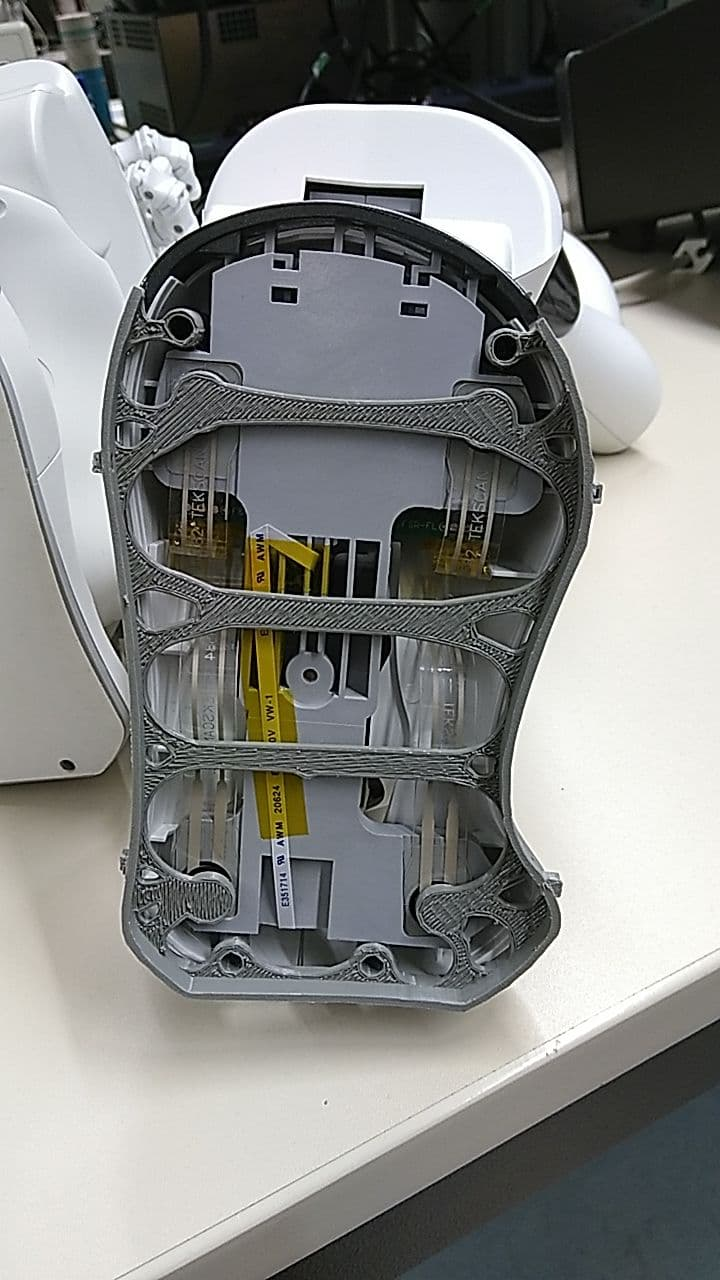
\includegraphics[width=\linewidth]{Bilder/Schuh_an_NAO_ohne_Sohle.jpg}
	\end{subfigure}
	\hfill
	\begin{subfigure}[c]{0.622\linewidth}
		\centering
		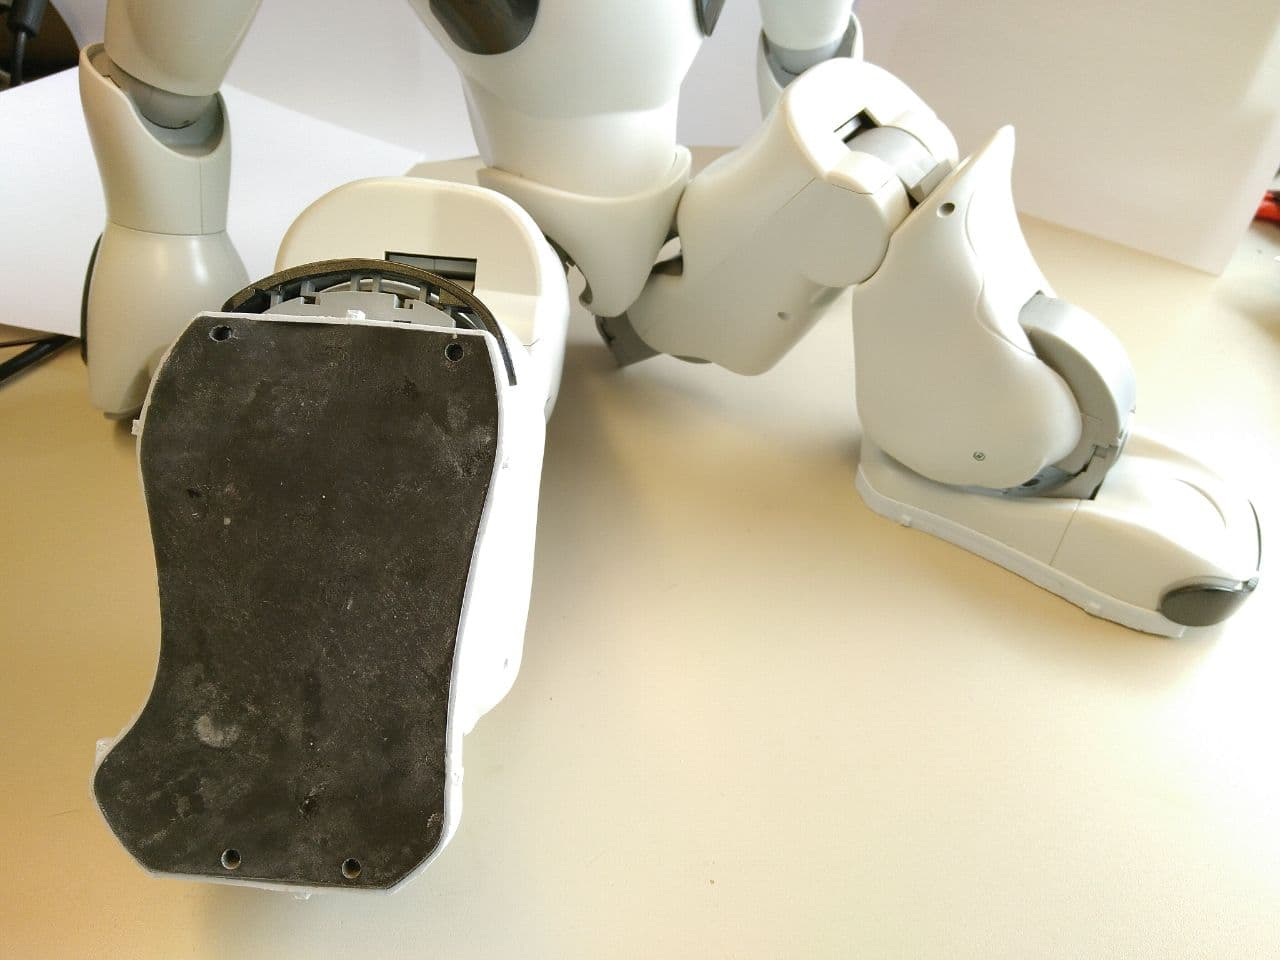
\includegraphics[width=\linewidth]{Bilder/Schuh_an_NAO_mit_Sohle.jpg}
	\end{subfigure}
	\hfill
	\caption{\textit{Links:} Der in Abb. \ref{Schuh_Inventor} in Autodesk Inventor erstellte Schuh aus PETG befestigt an der Unterseite des Fußes von NAO. \textit{Rechts:} Die aus der Gussform aus Abb. \ref{Gussform_Inventor} entnommene Sohle mit 20\,\% MAP Anteil befestigt in dem aus PETG gedruckten Schuh.}
	\label{nao_mit_schuhen}
\end{figure}

\begin{figure}[tb]
	\hfill
	\begin{subfigure}[c]{0.4\linewidth}
		\centering
		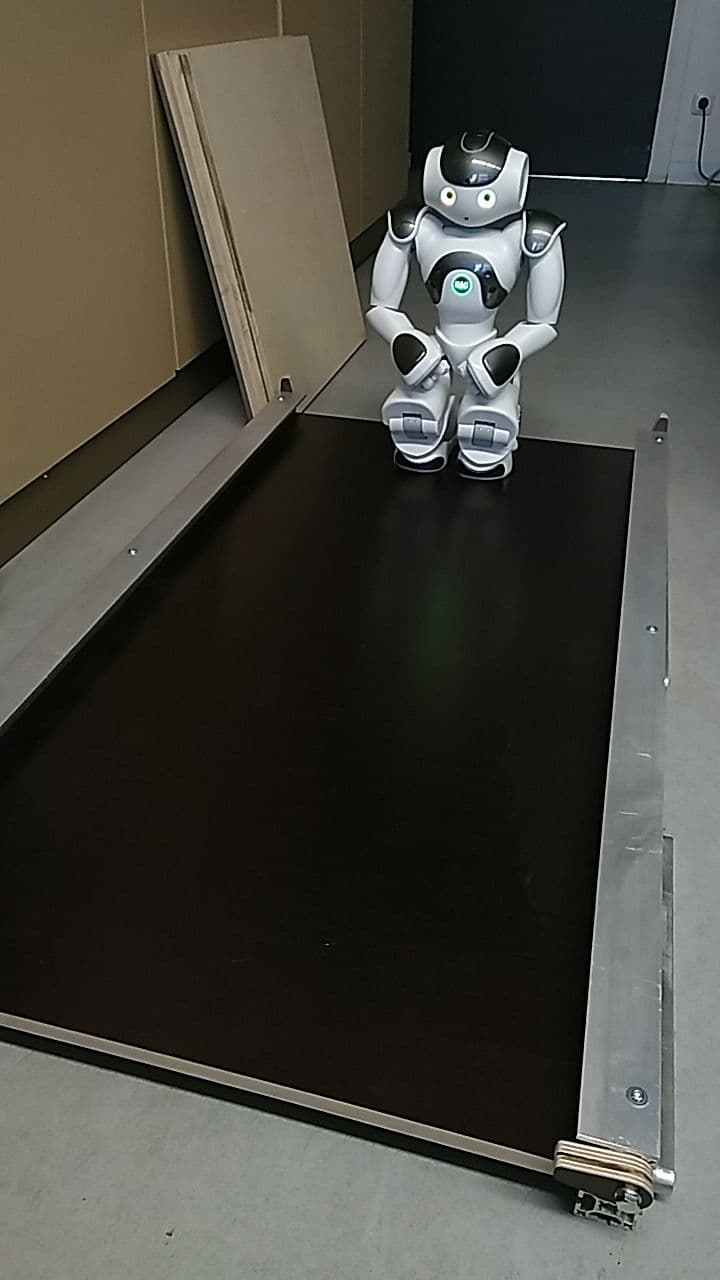
\includegraphics[width=\linewidth]{Bilder/NAO_auf_Rampe2.jpg}
	\end{subfigure}
	\hfill
	\begin{subfigure}[c]{0.4315\linewidth}
		\centering
		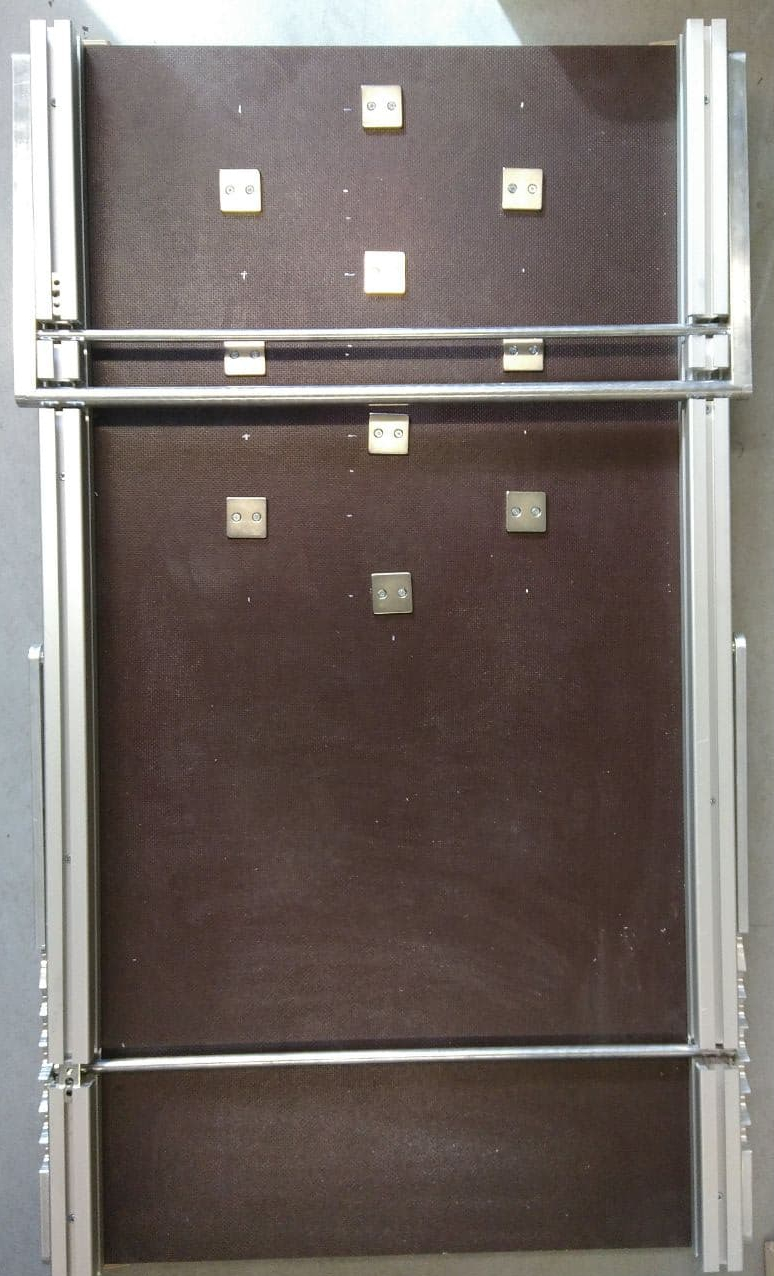
\includegraphics[width=\linewidth]{Bilder/magneten_an_rampe1_geschnitten.jpg}
	\end{subfigure}
	\hfill
	\caption{\textit{Links:} Der NAO Roboter steht im Ruhezustand an der Startposition auf der Rampe ohne Einlageplatten (an der Wand links neben NAO). \textit{Rechts:} Rampenunterseite mit befestigten Neodymmagneten.}
	\label{nao_und_rampe}
\end{figure}


% Bilder des tatsächlichen Versuchaufbaus.
% 
\FloatBarrier
\newpage
\section{Auswertung und Interpretation}
In diesem Kapitel werden die aufgenommenen Messungen ausgewertet und deren Bedeutung graphisch analysiert. Hierbei werden die Aufnahmen von zwei dimensionalen Ausgaben, welche das Gleichgewicht des Roboters widerspiegeln und die Werte der Aktoren in den Gelenken unterschieden.

\subsection{Gleichgewichtssensoren}

Wie in Kapitel \ref{software} beschrieben, werden zwei dimensionale Ausgaben, wie die x- und y-Ausgabe des Gyroskops, in einem Scatterhistogramm dargestellt, welches es ermöglicht, die Dichteverteilung einzusehen. 

\begin{figure}[b!]
	\centering
	\begin{adjustwidth}{-0.2\linewidth}{-0.2\linewidth}
		\hspace{+35pt}
		\begin{subfigure}[c]{.5\linewidth}
			\centering
			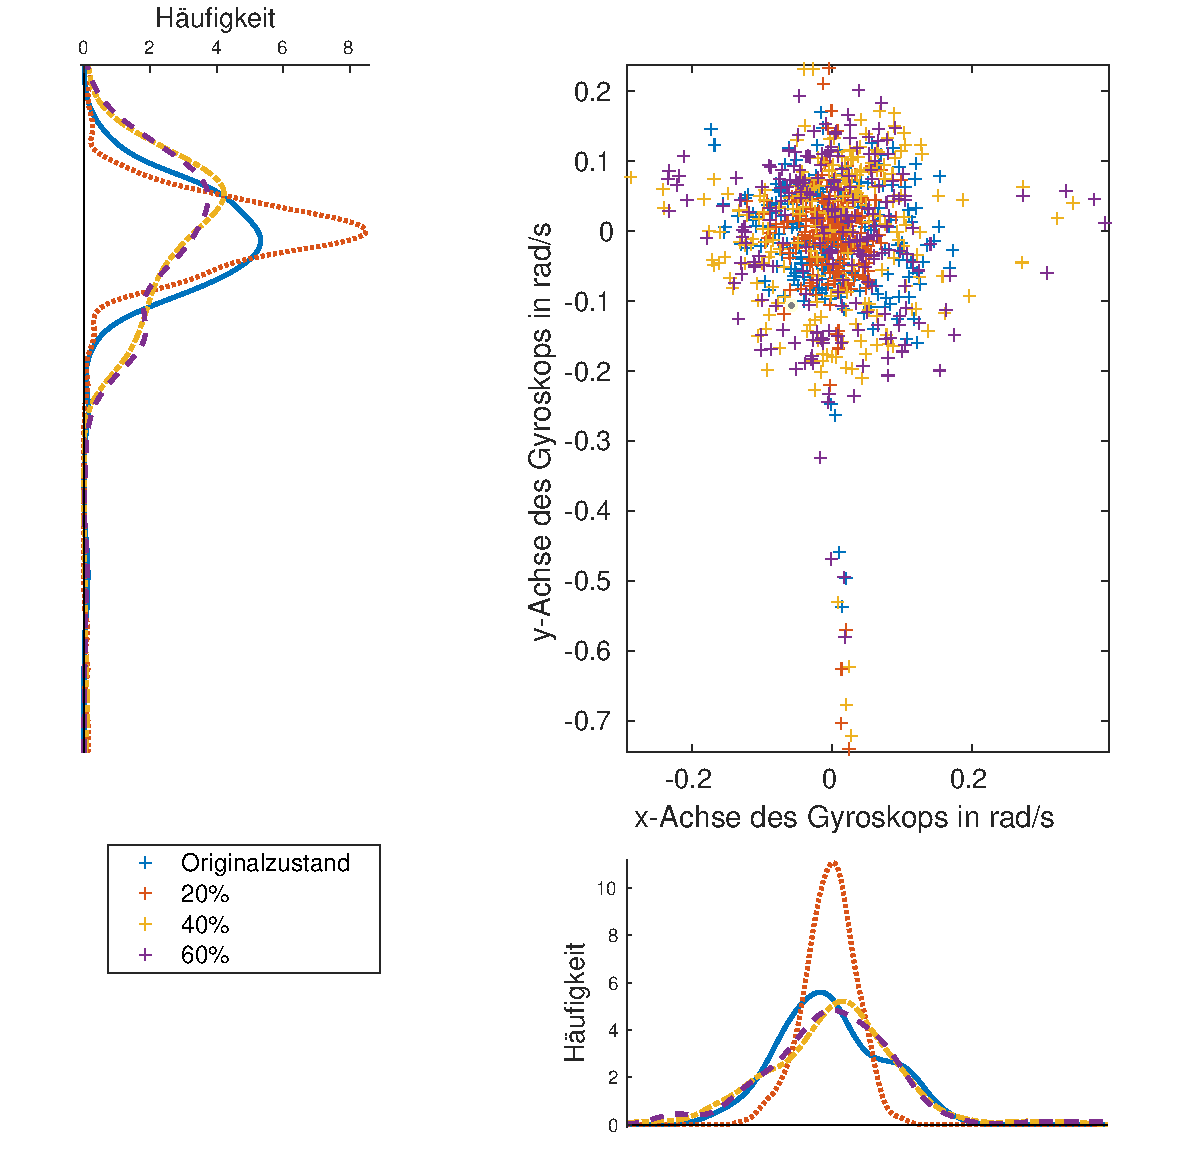
\includegraphics[width=\linewidth]{Bilder/Gyr_Grund_20_40_60_ohneM.pdf}
			\vspace{5pt}
		\end{subfigure}
		\hspace{-35pt}
		\begin{subfigure}[c]{.5\linewidth}
			\centering
			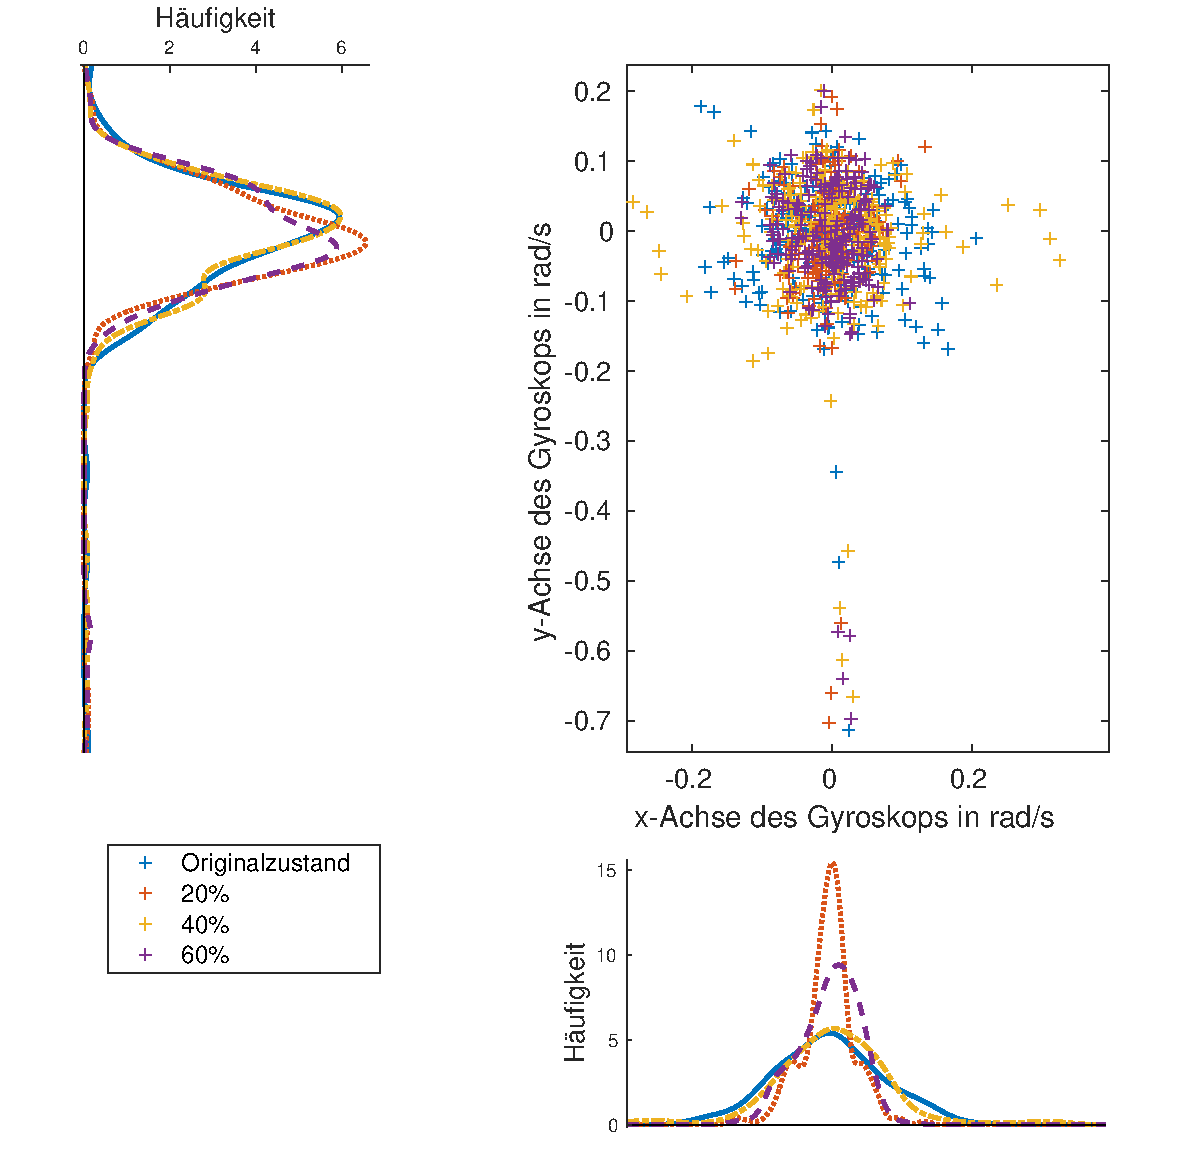
\includegraphics[width=\linewidth]{Bilder/Gyr_Grund_20_40_60_mitM.pdf}
			\vspace{5pt}
		\end{subfigure}
	\end{adjustwidth}
	\caption{Ausgabe des Gyroskops, x-Achse auf y-Achse, links ohne Magneten, rechts mit Magneten}\label{Gyr}
\end{figure}

In Abb. \ref{Gyr} sind die Aufnahmen des Gyroskops zu erkennen. Jede Ausgabe besteht aus 220 Punkten, da dies die Anzahl der Messdurchläufe pro Lauf sind. Jeder Wert wurde durch das arithmetische Mittel aus Gleichung \eqref{mean} aller Messpunkte zu diesem Zeitpunkt ermittelt. Der Graph auf der linken Seite ist die Ausgabe für die Messungen ohne Magneten an der Rampenunterseite, auf der rechten Seite die für die Messungen mit Magneten. Die jeweils zwei errechneten Dichteverteilung am linken und am unteren Rand des Hauptplots spiegeln die Verteilung des Scatterplots eindimensional wider. Die vereinzelten Punkte unterhalb von $-0,3 \unit{rad/s}$ sind dem Beginn der Messung geschuldet, während derer NAO sich in aufrechtem Stand befindet. Sobald der Roboter die laufende Haltung einnimmt, wird der Torso deshalb relativ schnell bewegt. Dies wird während der restlichen Aufnahmen nur passieren, wenn NAO umfällt. 
%Sollte ich hierfür das Gyroskop einmal auf die Zeit gesehen zeigen?

% abb 13: wie sind die Graphen aufgeteilt, was haben die Graphen an der seite zu bedeuten. Warum sind da vereinzelnd punkte in der mitte unten

Bei einem stabilen Gang würde man erwarten, dass die Geschwindigkeit, in der sich der Torso bewegt, gering bleibt. Dies bedeutet, je mehr Ausschwankungen zu sehen sind, desto instabiler läuft dieser Roboter und desto eher würde er das Gleichgewicht verlieren. 
% was würde man erwarten, wenn NAO stabil läuft

In Abb. \ref{Gyr} ist eine Tendenz von stabiler werdendem Gang von ohne Magneten zu mit Magneten zu erkennen. Allerdings fällt dies auch für den Originalschuh auf, welcher kein MAP enthält. Grund hierfür könnte der etwa 1cm breite Magnet sein, welcher den unteren Teil des Schuhs in Stellung hält, bevor die Schrauben zur Befestigung verwendet werden.

Des Weiteren heben sich die Sohlen mit $20\,\%$ CIP Anteil besonders hervor. Durch die Magneten erfahren sie ebenfalls eine minimale Verbesserung. Hierbei sollte erwähnt werden, dass diese Sohle mit der gedruckten Halterung dem Gewicht der Originalsohle am nächsten kommt und dadurch die Stabilität vielleicht besser gewährleistet ist. Die stärkste Auswirkung sowohl für die x- als auch die y-Achse gab es für $60\,\%$ CIP Anteil. Dies ist nicht verwunderlich, da hier die größte magnetische Kraft wirkt. 
% erst dann: man sieht eine Tendenz, dass es mit Magneten stabiler ist. 20% ist von vorn herein sehr stabil, der Grundschuh sowie 40% zeigen zeigt in y-Achse eine starke verbesserung mit Magneten, 60% zeigt in allen Achsen eine Verbesserung der Stabilität

\begin{figure}[htb]
	\centering
	\begin{adjustwidth}{-0.2\linewidth}{-0.2\linewidth}
		\hspace{+45pt}
		\begin{subfigure}[c]{.45\linewidth}
			\centering
			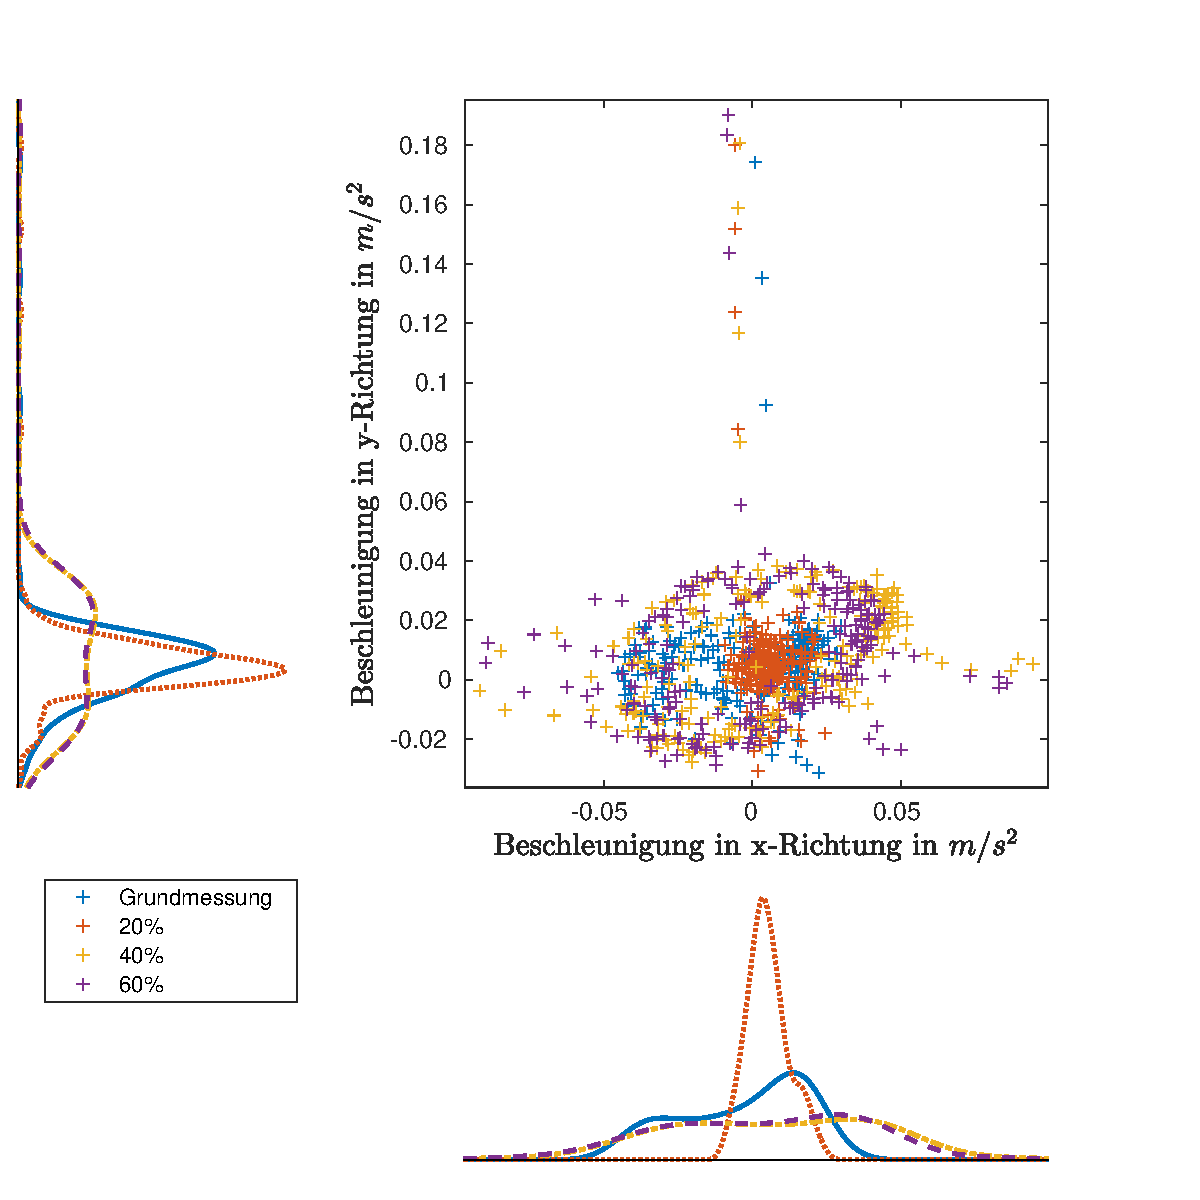
\includegraphics[width=\linewidth]{Bilder/Beschleunigung_Grund_20_40_60_ohneM.pdf}
			\vspace{5pt}
		\end{subfigure}
		%\hfill
		\hspace{-25pt}
		\begin{subfigure}[c]{.45\linewidth}
			\centering
			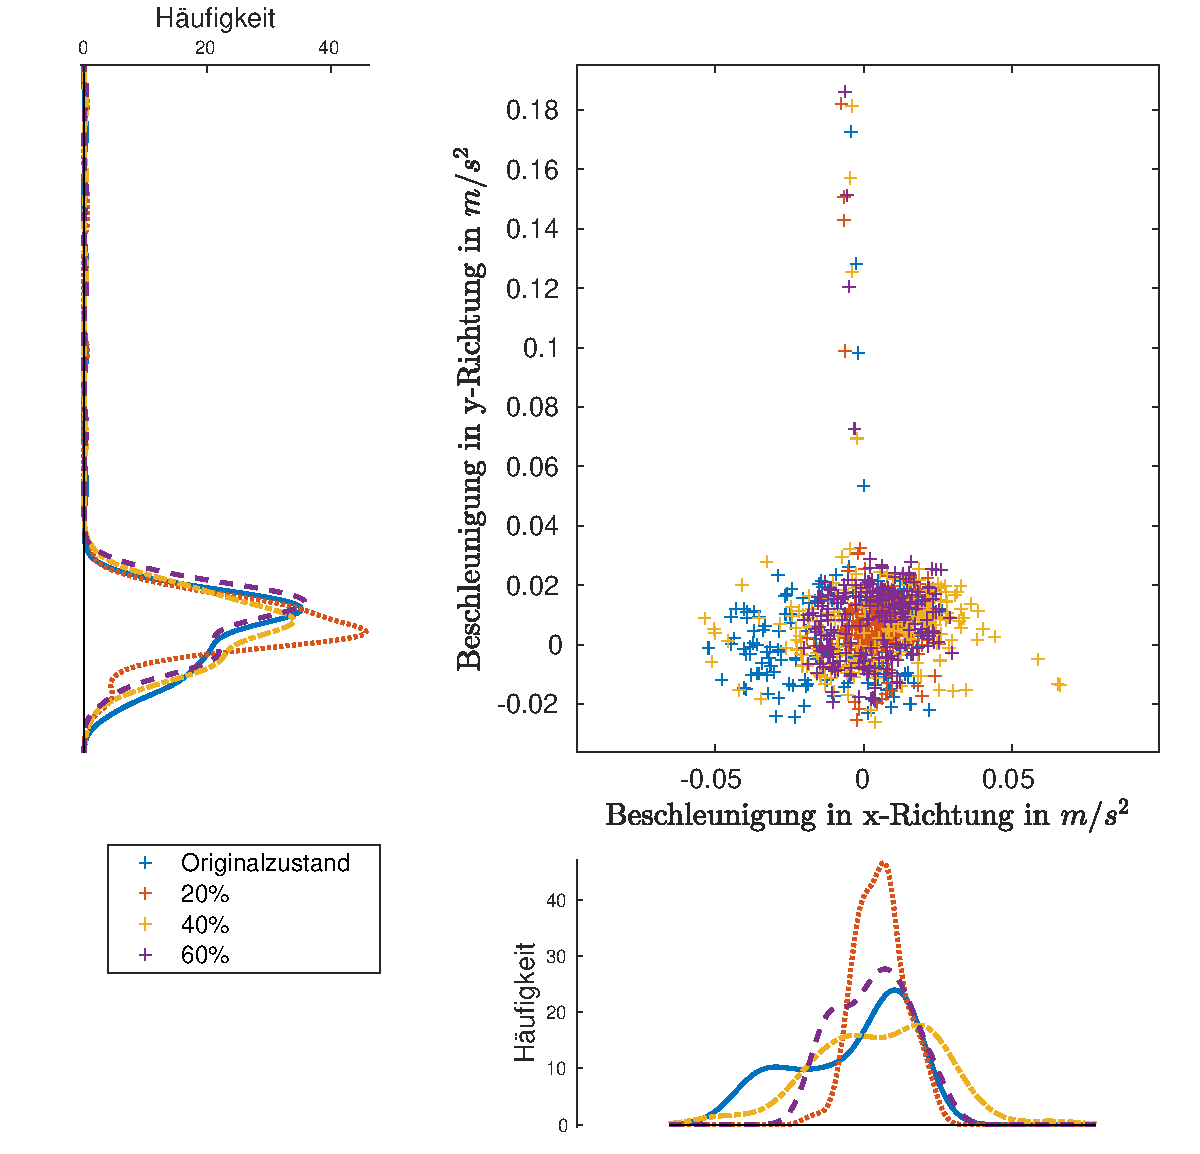
\includegraphics[width=\linewidth]{Bilder/Beschleunigung_Grund_20_40_60_mitM.pdf}
			\vspace{5pt}
		\end{subfigure}
	\end{adjustwidth}
	\caption{Ausgabe des Beschleunigungssensors, x-Achse auf y-Achse aufgetragen, links ohne Magneten, rechts mit Magneten} \label{Acc}
\end{figure}
Die Beschleunigungssensoren messen wie bereits erwähnt in $\unit{m/s^2}$ die Beschleunigung des Torsos. Deshalb ist ebenfalls zu erwarten, dass bei einem stabilen Gang diese Werte sich in der Nähe des Nullpunkts zentrieren, sollte NAO stabil laufen. Genau wie in Abb. \ref{Gyr} zeigen die Graphen in Abb. \ref{Acc} eine Tendenz zu einem stabileren Lauf mit Magneten. Auch hier wirken die $20\,\%$igen Proben außergewöhnlich stabil, während die $60\,\%$igen Proben in x-Richtung von den Magneten am meisten Profitieren. Gleichzeitig verhalten sich $40$ zu $60\,\%$ in y-Richtung ähnlich. 
% abb 14: Gleiche Graphenaufteilung, ähnliches Ergebnis

\begin{figure}[tb]
	\centering
	\begin{adjustwidth}{-0.2\linewidth}{-0.2\linewidth}
		\hspace{45pt}
		\begin{subfigure}[c]{.45\linewidth}
			\centering
			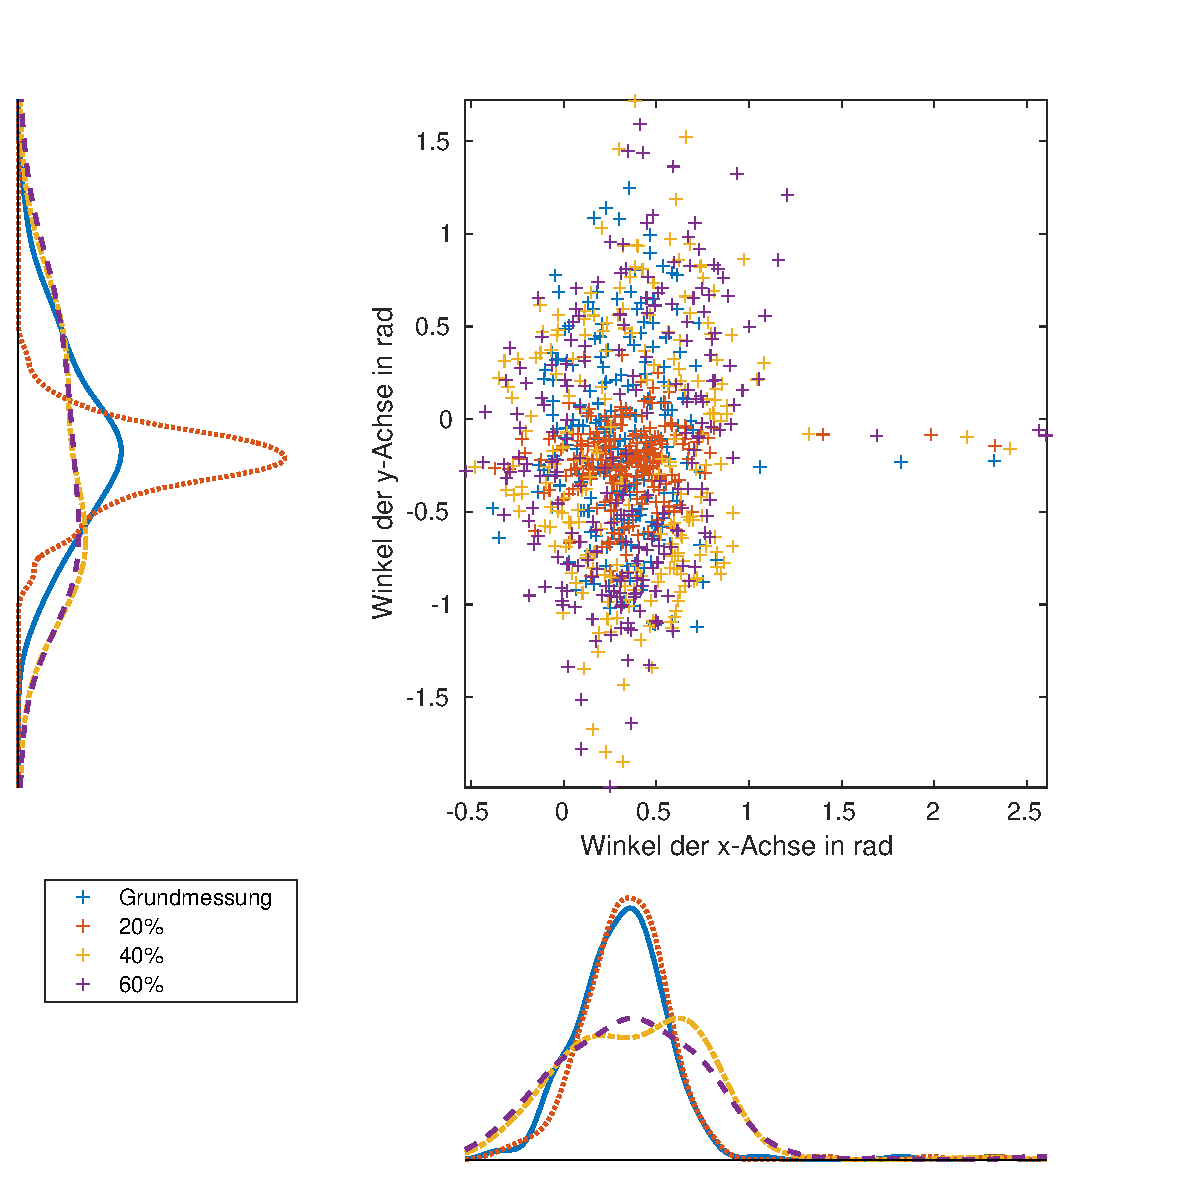
\includegraphics[width=\linewidth]{Bilder/Winkel_Grund_20_40_60_ohneM.pdf}
			\vspace{5pt}
		\end{subfigure}
		\hspace{-20pt}
		%\hfill
		\begin{subfigure}[c]{.45\linewidth}
			\centering
			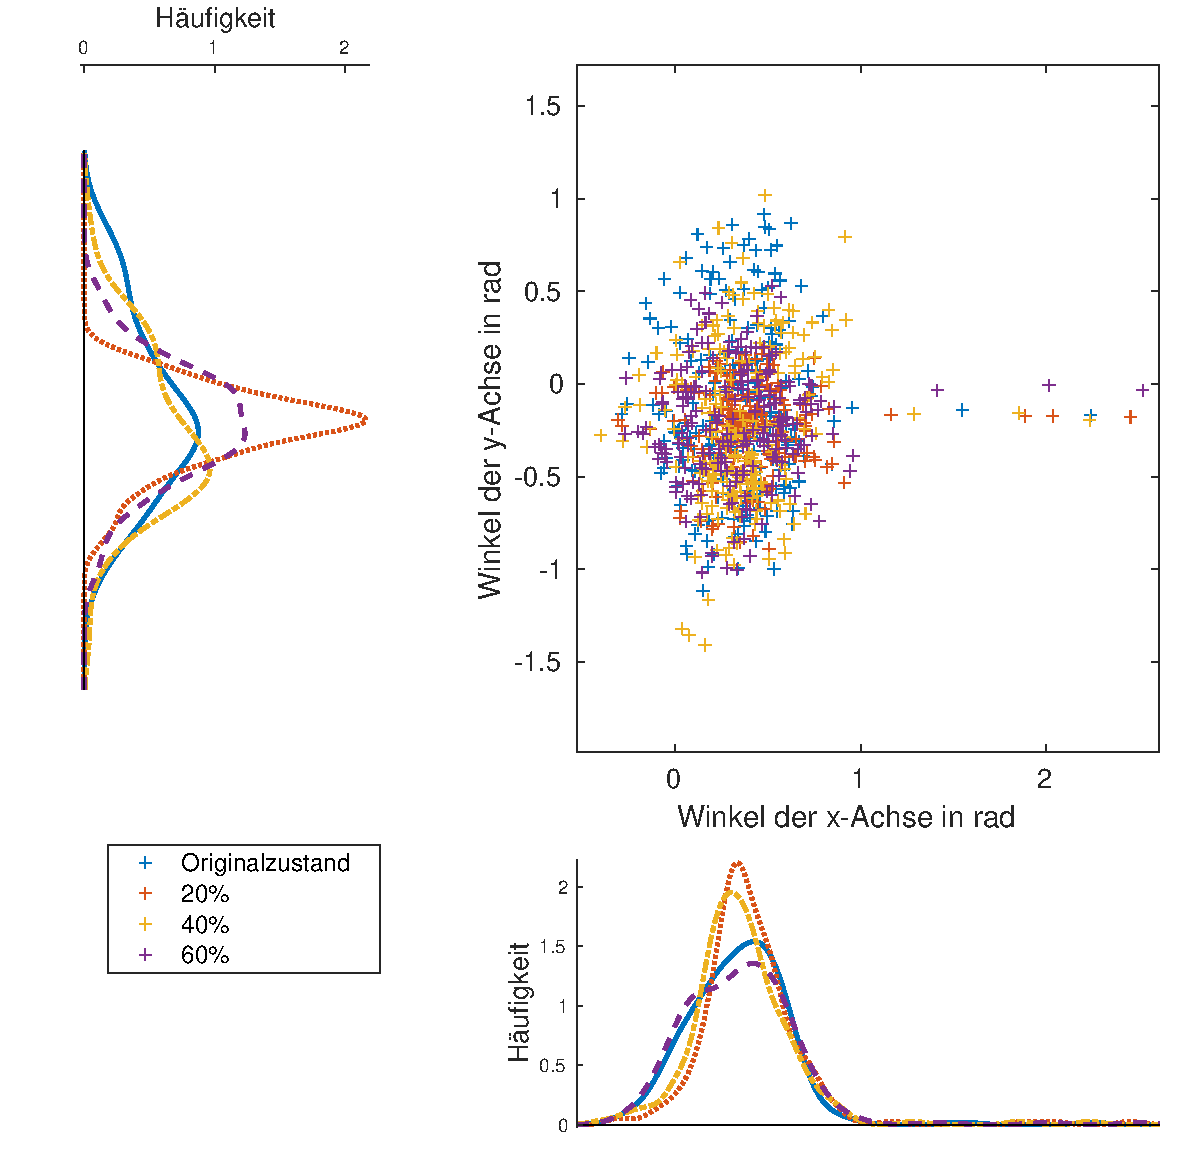
\includegraphics[width=\linewidth]{Bilder/Winkel_Grund_20_40_60_mitM.pdf}
			\vspace{5pt}
		\end{subfigure}
	\end{adjustwidth}
	\caption{Echtzeit errechneter Winkel, x-Achse auf y-Achse aufgetragen, links ohne Magneten, rechts mit Magneten} \label{Angle}
\end{figure}
Die Winkelwerte in Abb. \ref{Angle} entstehen aus der Berechnung durch Gyroskop und Beschleunigungssensor. Da beide alle Graphen zuvor eine Tendenz von höherer Stabilität durch Magneten aufwiesen, ist zu erwarten, dass dies bei den Winkelgraphen auch der Fall ist. In der y-Achse ist eine Verbesserung von $40$ und $60\,\%$ erkennbar.In x-Richtung scheint $40\,\%$iges MAP am meisten zu profitieren, allerdings gilt für den Originalschuh eher das Gegenteil. 
% abb 15: Ist aus den Werten, welche in abb 13 und 14 zu sehen sind errechnet. deshalb auch hier ähnliches Ergebnis

\begin{figure}[tb]
	\centering
	\begin{adjustwidth}{-0.2\linewidth}{-0.2\linewidth}
		\hspace{40pt}
		\begin{subfigure}[c]{.45\linewidth}
			\centering
			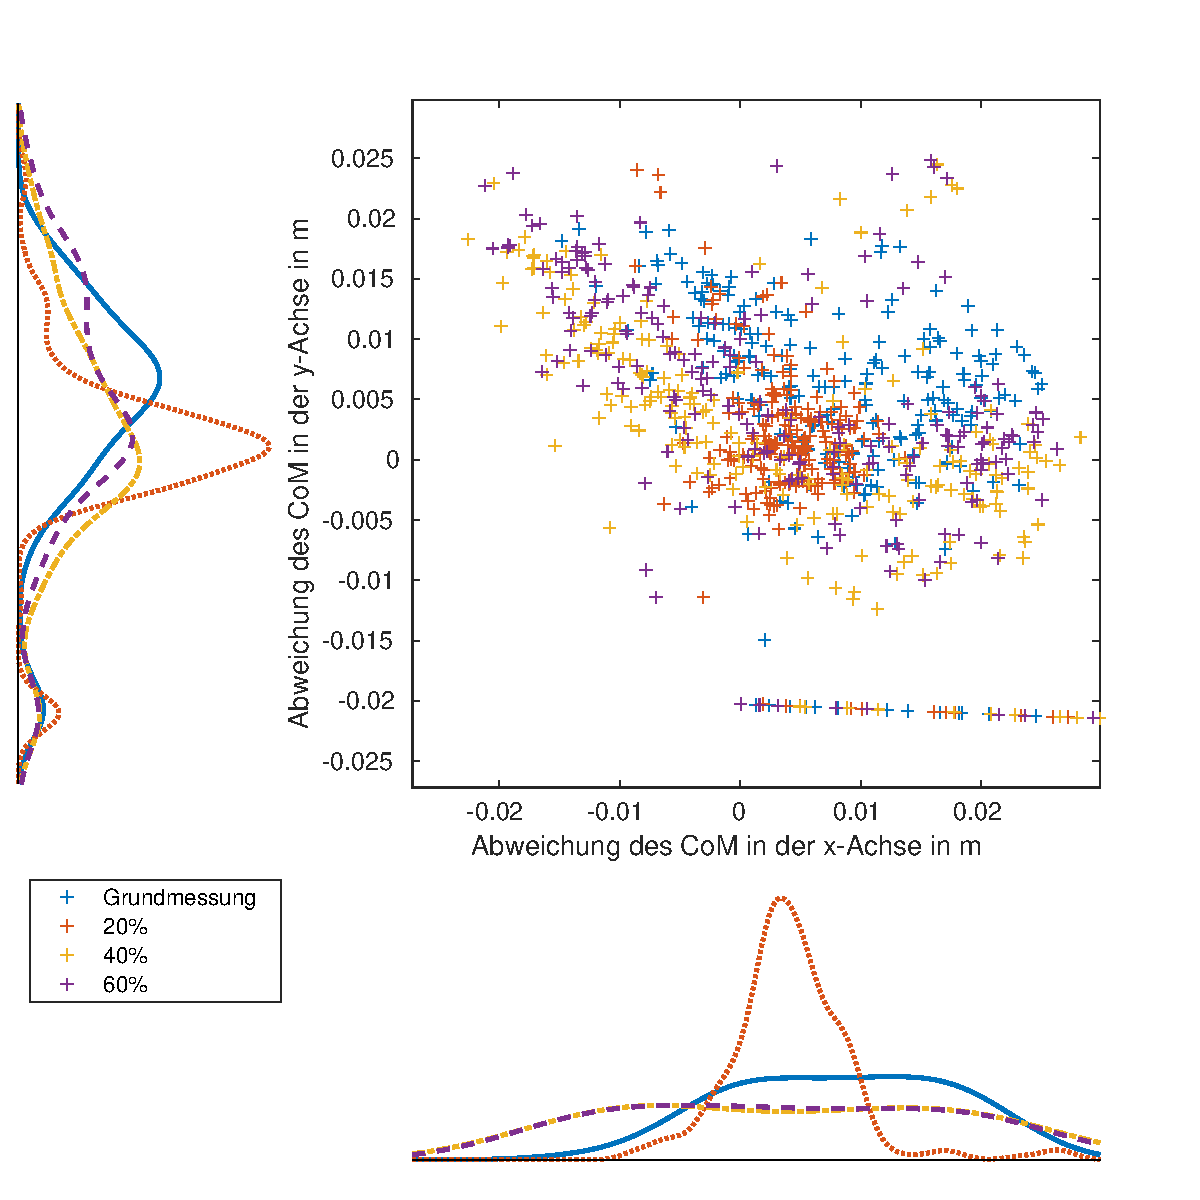
\includegraphics[width=\linewidth]{Bilder/links_CoM_ohneM.pdf}
			\vspace{5pt}
		\end{subfigure}
		\hspace{-10pt}
		%\hfill
		\begin{subfigure}[c]{.45\linewidth}
			\centering
			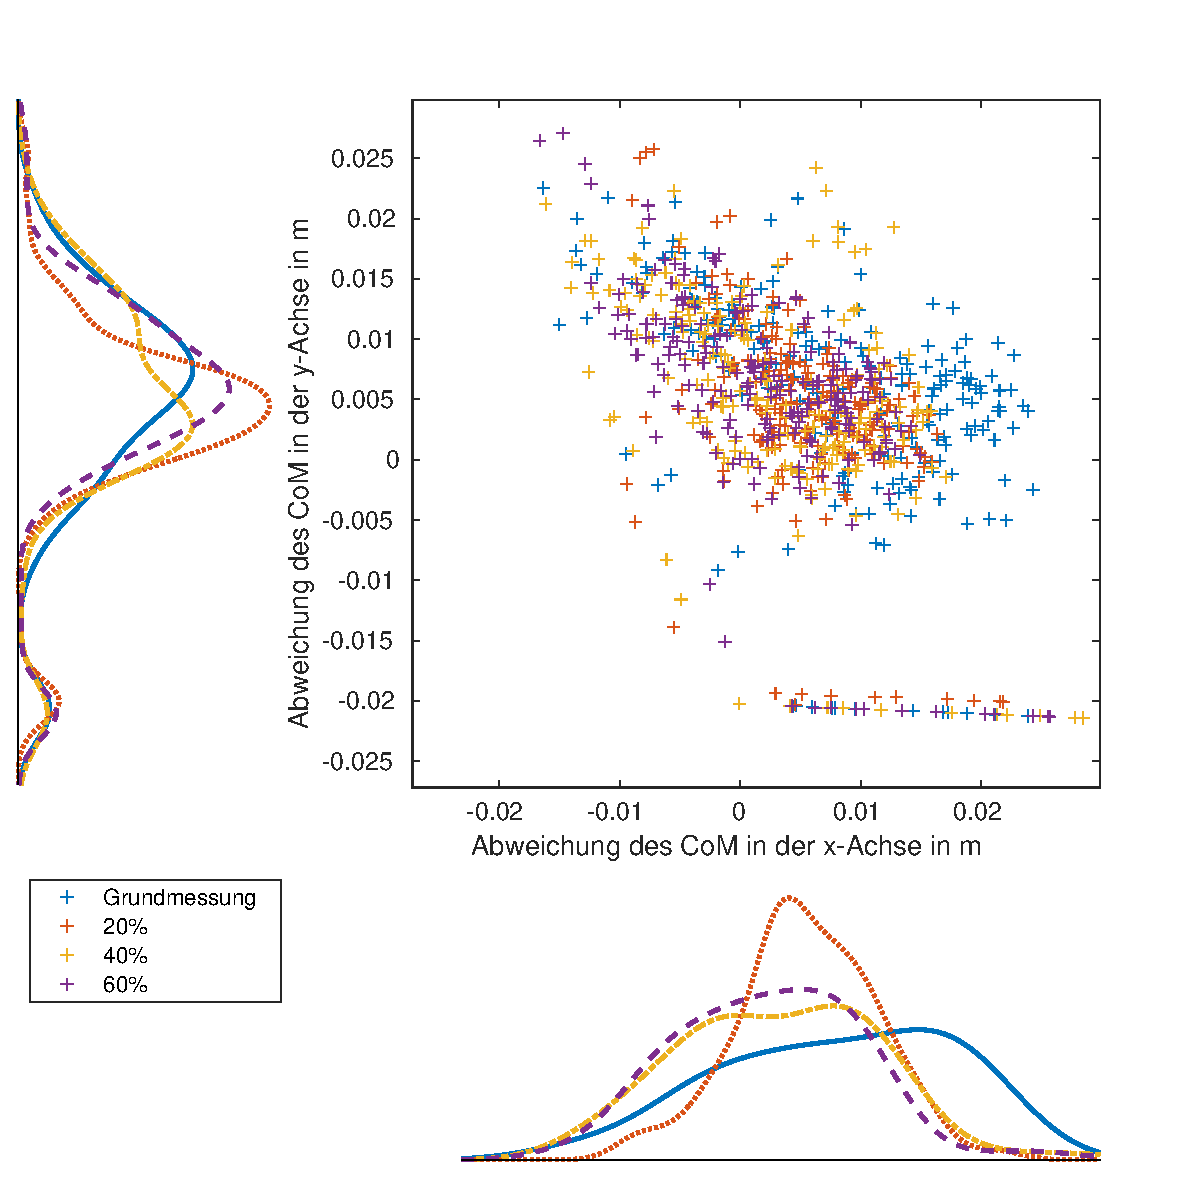
\includegraphics[width=\linewidth]{Bilder/links_CoM_mitM.pdf}
			\vspace{5pt}
		\end{subfigure}
	\end{adjustwidth}
	\caption{Linker errechneter Massenschwerpunkt aufgenommen durch die FSR, x-Achse auf y-Achse aufgetragen, links ohne Magneten, rechts mit Magneten} \label{CoM_links}
\end{figure}
\begin{figure}[tb]
	\centering
	\begin{adjustwidth}{-0.2\linewidth}{-0.2\linewidth}
		\hspace{40pt}
		\begin{subfigure}[c]{.45\linewidth}
			\centering
			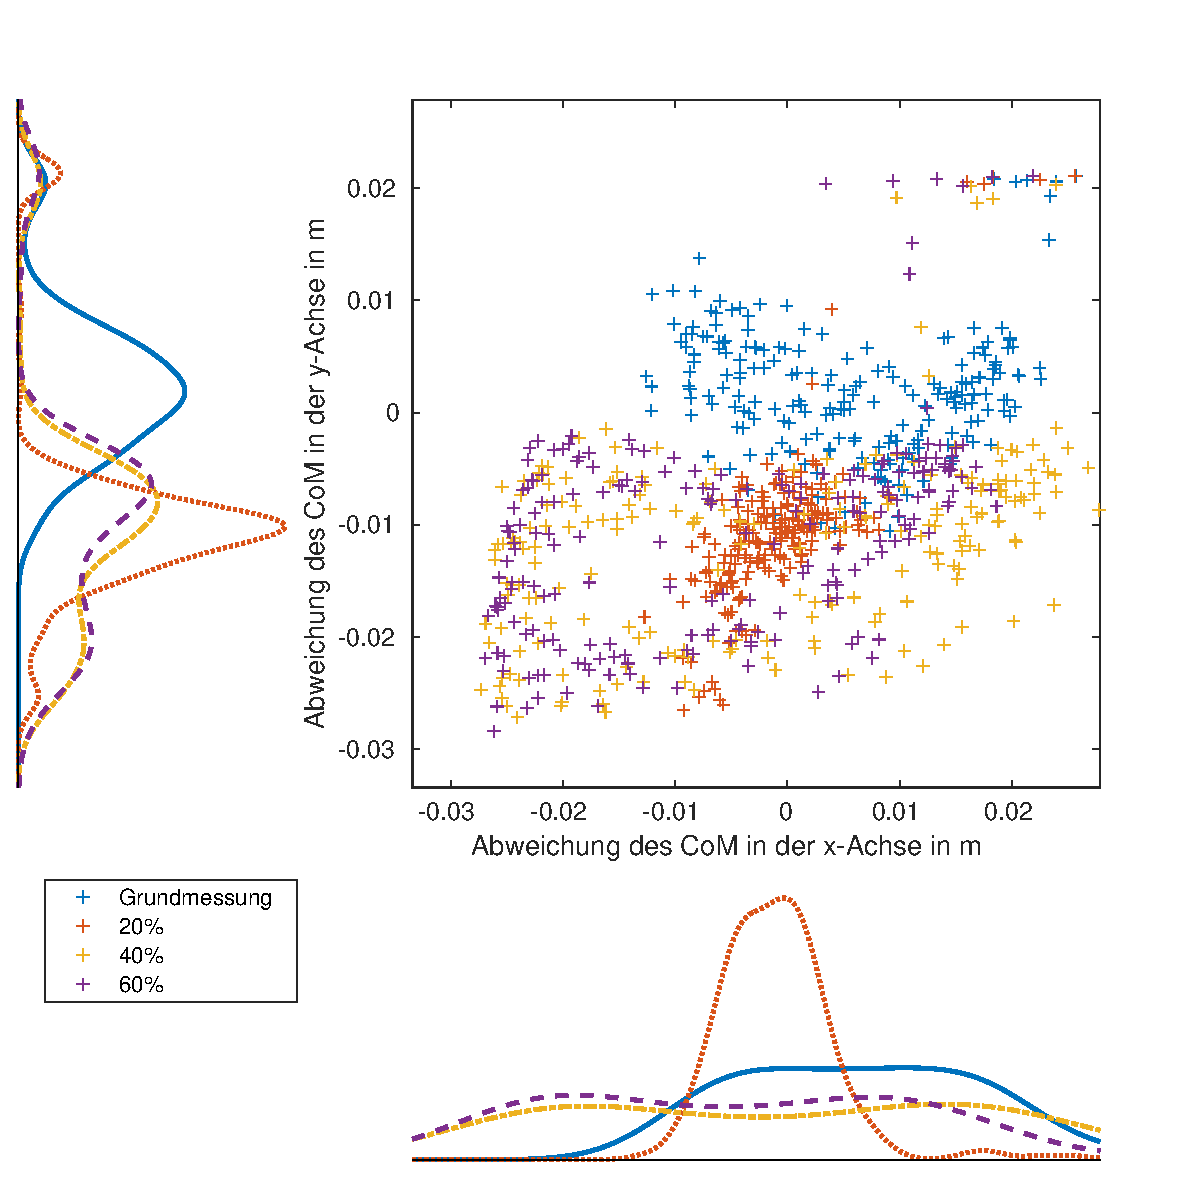
\includegraphics[width=\linewidth]{Bilder/rechts_CoM_ohneM.pdf}
			\vspace{5pt}
		\end{subfigure}
		\hspace{-10pt}
		%\hfill
		\begin{subfigure}[c]{.45\linewidth}
			\centering
			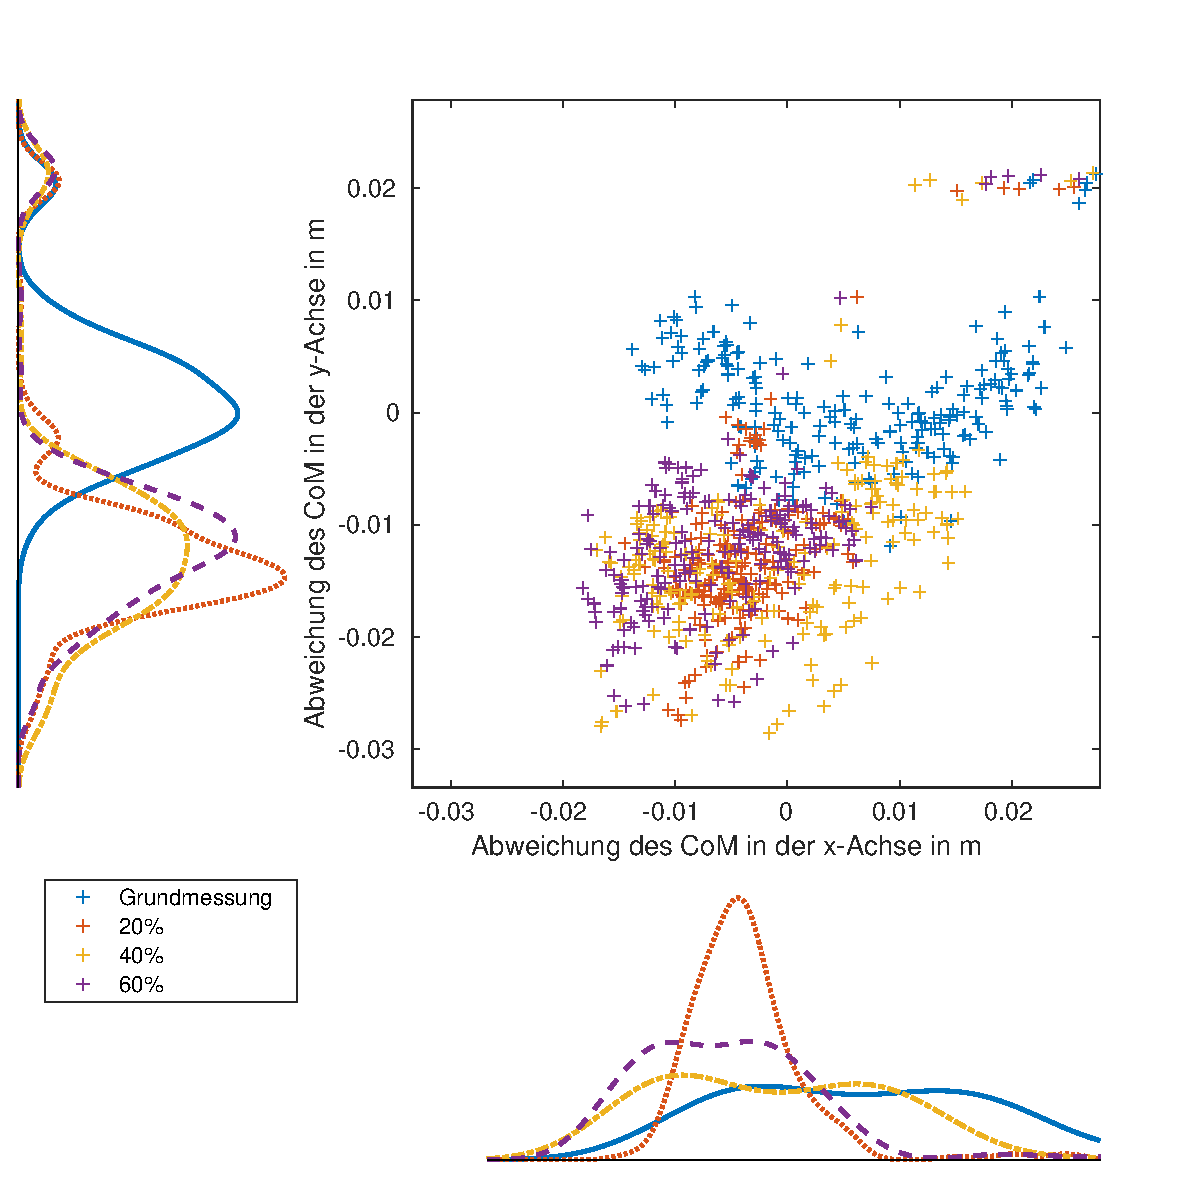
\includegraphics[width=\linewidth]{Bilder/rechts_CoM_mitM.pdf}
			\vspace{5pt}
		\end{subfigure}
	\end{adjustwidth}
	\caption{Rechter errechneter Massenschwerpunkt aufgenommen durch die FSR, x-Achse auf y-Achse aufgetragen, links ohne Magneten, rechts mit Magneten} \label{CoM_rechts}
\end{figure}
Das hier verwendete Modell von NAO bietet noch die Möglichkeit die Stabilität des Gangs über die Drucksensoren in den Fußsohlen, auf die in Kapitel \ref{aufbau_NAO} bereits eingegangen wurde, zu messen. Die errechneten Werte der zweidimensionalen Massenschwerpunkte durch die 8 FSR Sensoren sind in Abb \ref{CoM_links} und \ref{CoM_rechts} zu sehen.
% abb 16 und 17 sind aus den FSR Daten entstanden und weißen eine ebenfalls weisen nur für die MAP sohlen unterschiede auf, aber kaum für den Grundschuh. 

% Warum diese Auswertung mit Vorsicht zu genießen ist: frühere Auswertung
% Ungenauigkeiten der FSR
% Dennoch wird bei allen Graphen eine verbesserung mit Magneten festgestellt, warum könnte das so sein?


%Notizen:
%
%Die folgenden Graphen unterscheiden sich in ihrer Darstellung: Zum einen wurden Gyroskop, Beschleunigungssensors, Winkel und Center of Mass in sog. Scatterhistogrammen geplottet, siehe Abb \ref{Gyr},\ref{Acc},\ref{Angle}. Der Hauptplot ist ein scatter-Plot, welcher die Verteilung auf der X verglichen zur Y-Achse zeigt. An den Rändern sind jeweils die Histogramme der Achsen aufgetragen, welche die Wahrscheinlichkeitsverteilung angeben. Dabei ist die Annahme, dass ein stabilierer Gang eine steilere Wahrscheinlichkeitsverteilung hervorbringt, da sich die Aufnahmepunkte in der Mitte häufen müssten. Eine flache Verteilungskurve würde im Gegenzug bedeuten, dass NAO während dem Gang große Schwankungen aufweist und deshalb instabiler läuft.
%
%Es lässt sich eine Tendenz erkennen, dass der Gang mit Magneten stabiler ist, als ohne. Außerdem zeichnet sich das 20\,\% MAP durch besonders gute Stabilität hab. 
%
%Der Strom wurde in Histogrammen aufgetragen, welche die relative Häufigkeit des Stroms während der Messung aufzeigt. Die Graphen \ref{AnklePitch_Current_links},\ref{AnklePitch_Current_rechts},\ref{AnkleRoll_Current_links},\ref{AnkleRoll_Current_rechts} sind unterteilt in zwei Arten von Plots. Einerseits ist ein Histogramm mit jeweils 20 Säulen zu sehen. Diese wurde mit der Wahrscheinlichkeitsdichtefunktion von Matlab (pdf) ergänzt, um die Verteilung besser einsehen zu können.
%
%Die Annahme ist, dass ein höherer Strom mehr Reibungs- oder Haftwiderstand bedeuten. Leider ist die Datenlage hier sehr uneindeutig. 

\FloatBarrier
\subsection{Sensoren der Aktoren}

\begin{figure}[tb]
	\centering
%	\begin{adjustwidth}{-0.2\linewidth}{-0.2\linewidth}
%		\hspace{5pt}
		\begin{subfigure}[c]{.9\linewidth}
			\centering
			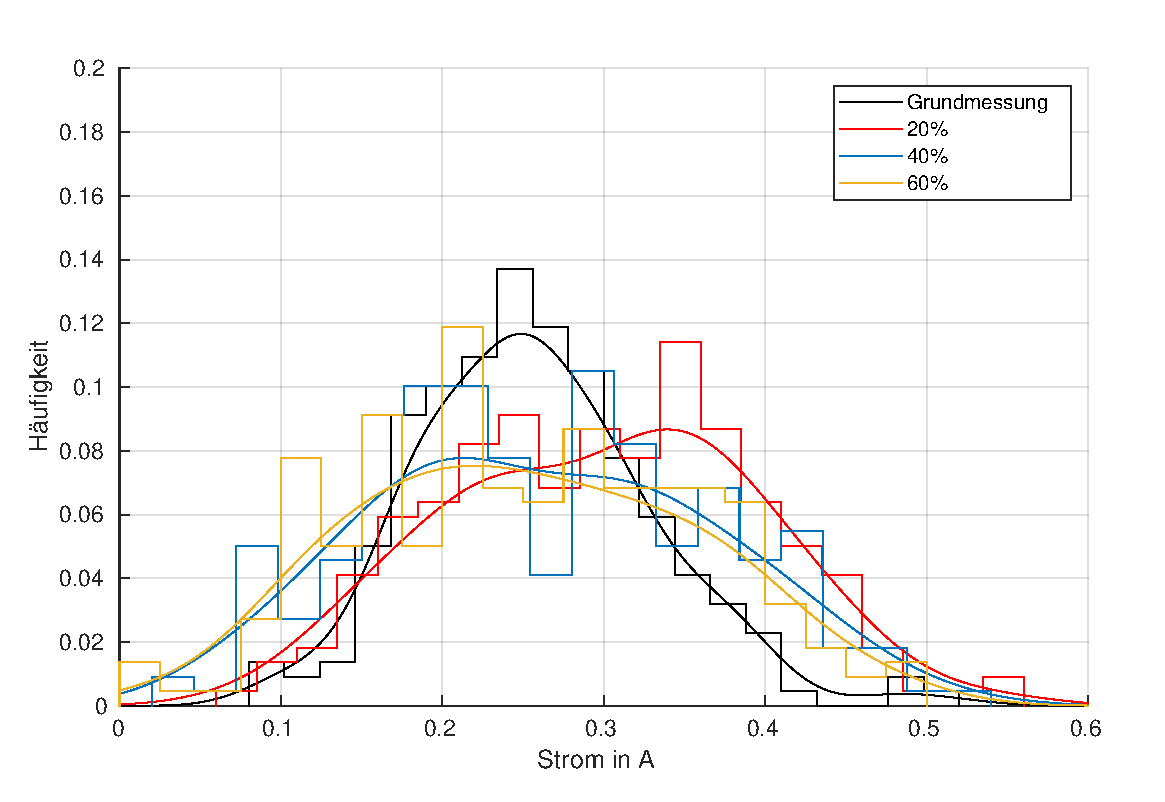
\includegraphics[width=\linewidth]{Bilder/links_Current_AnklePitch_ohneM.pdf}
%			\vspace{5pt}
		\end{subfigure}
%		\hspace{20pt}
%		\hfill
		\begin{subfigure}[c]{.9\linewidth}
			\centering
			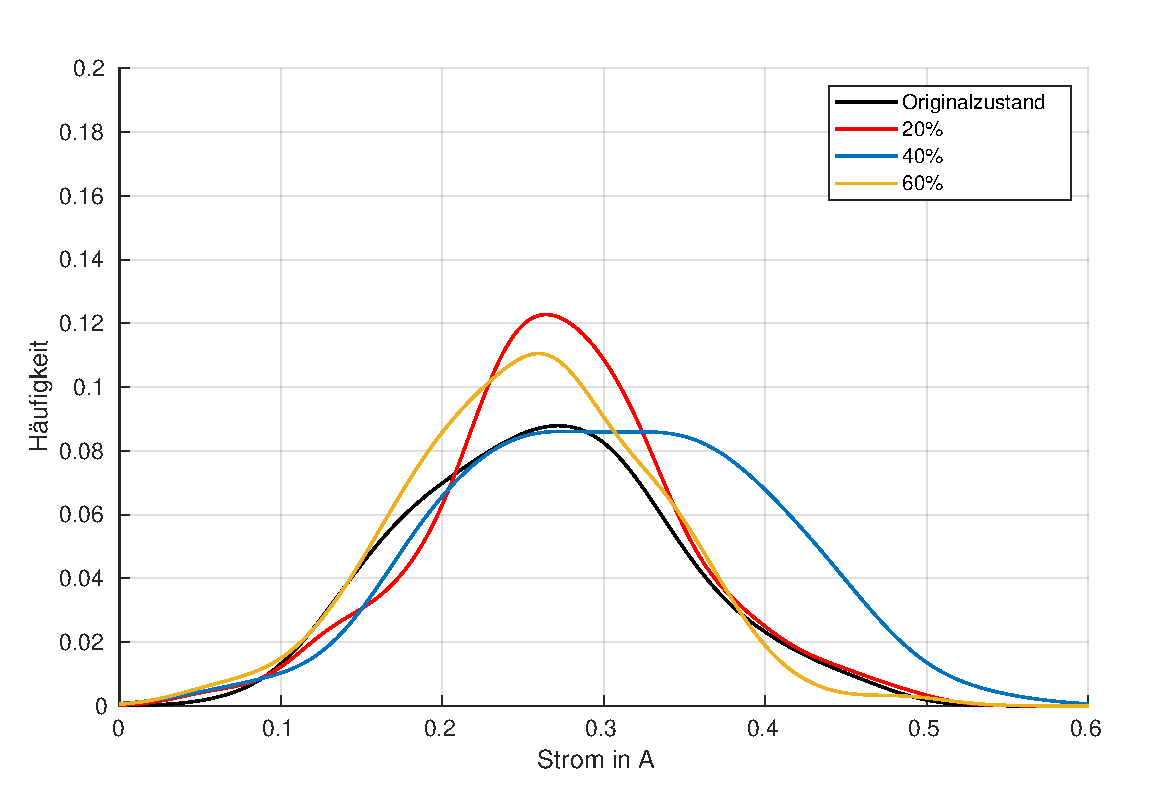
\includegraphics[width=\linewidth]{Bilder/links_Current_AnklePitch_mitM.pdf}
%			\vspace{5pt}
		\end{subfigure}
%	\end{adjustwidth}
	\caption{AnklePitch gemessener Strom im linken Fuß, Strom in Ampère aufgetragen auf die Häufigkeit. Das Histogramm wurde ergänzt durch eine Wahrscheinlichkeitsdichtefunktion. Der obere Graph sind die Aufnahmen ohne Magneten, der untere mit Magneten.} \label{AnklePitch_Current_links}
\end{figure}
\begin{figure}[tb]
	\centering
%	\begin{adjustwidth}{-0.2\linewidth}{-0.2\linewidth}
%		\hspace{5pt}
		\begin{subfigure}[c]{.9\linewidth}
			\centering
			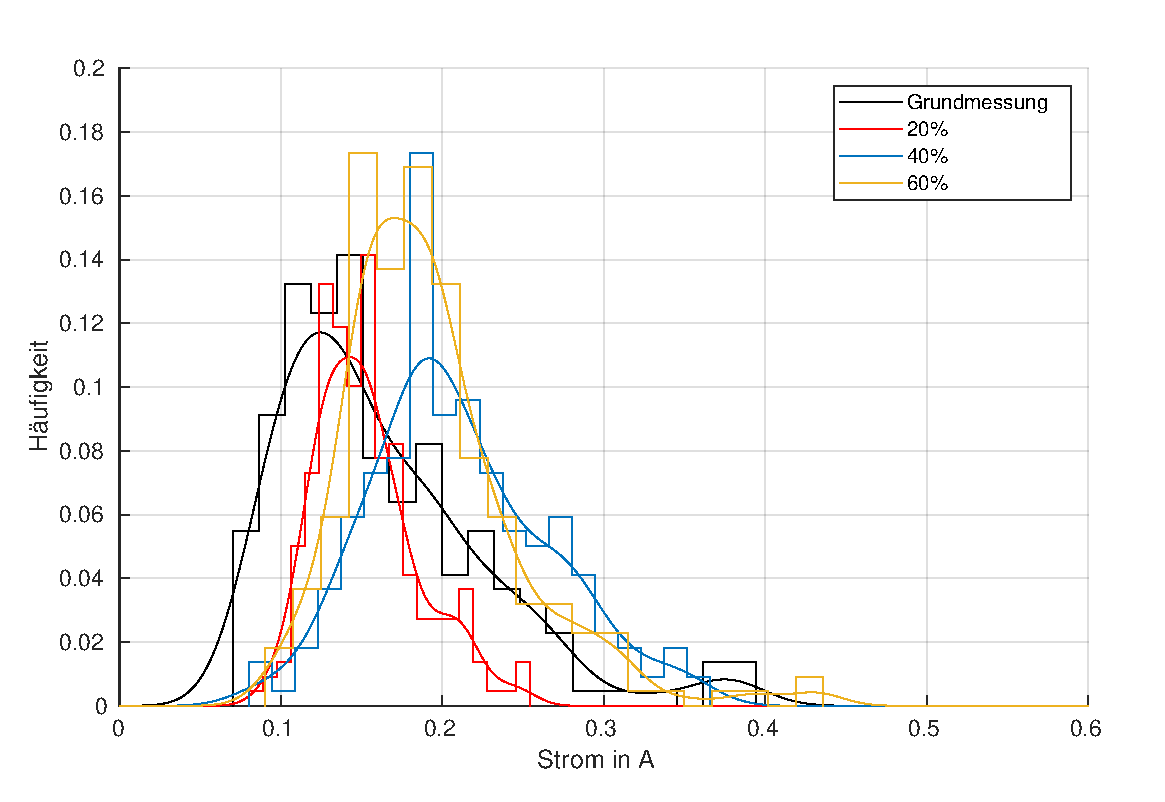
\includegraphics[width=\linewidth]{Bilder/rechts_Current_AnklePitch_ohneM.pdf}
			\vspace{5pt}
		\end{subfigure}
%		\hspace{20pt}
		\hfill
		\begin{subfigure}[c]{.9\linewidth}
			\centering
			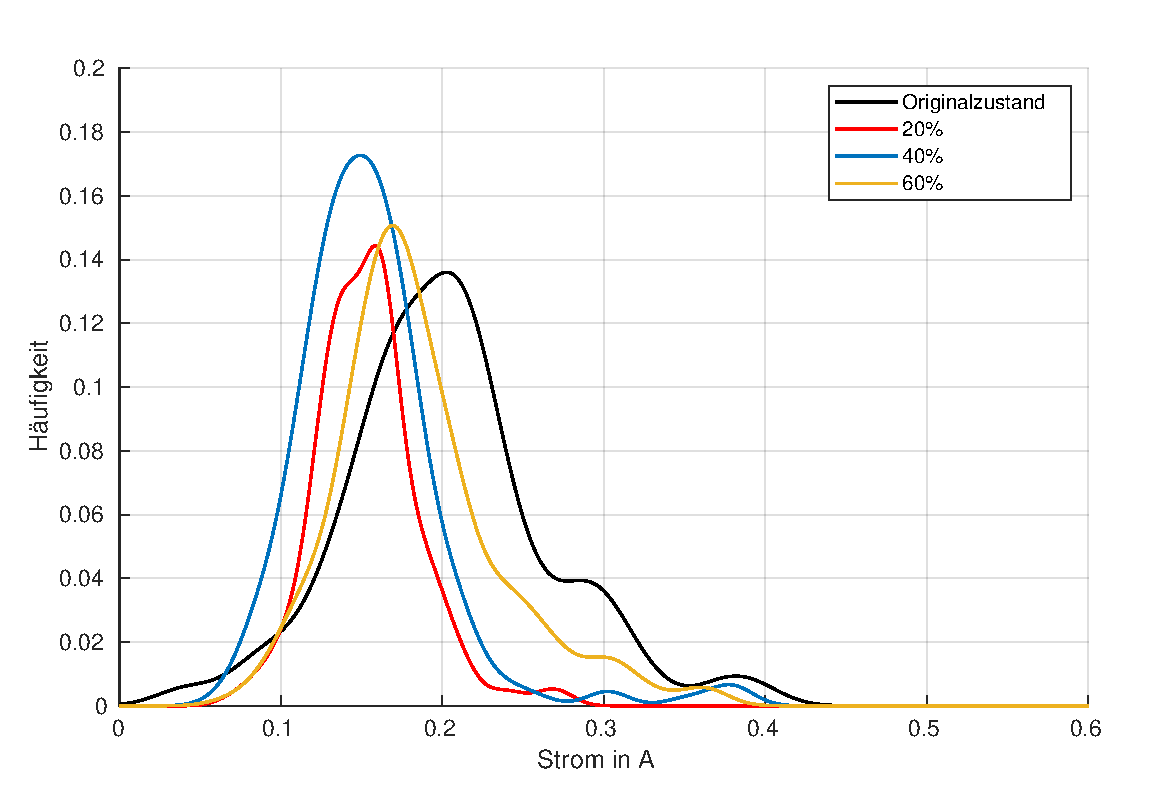
\includegraphics[width=\linewidth]{Bilder/rechts_Current_AnklePitch_mitM.pdf}
			\vspace{5pt}
		\end{subfigure}
%	\end{adjustwidth}
	\caption{AnklePitch gemessener Strom im rechter Fuß, Strom in Ampère aufgetragen auf die Häufigkeit. Das Histogramm wurde ergänzt durch eine Wahrscheinlichkeitsdichtefunktion. Der obere Graph sind die Aufnahmen ohne Magneten, der untere mit Magneten.} \label{AnklePitch_Current_rechts}
\end{figure}

\begin{figure}[tb]
	\centering
	%	\begin{adjustwidth}{-0.2\linewidth}{-0.2\linewidth}
	%		\hspace{5pt}
	\begin{subfigure}[c]{.9\linewidth}
		\centering
		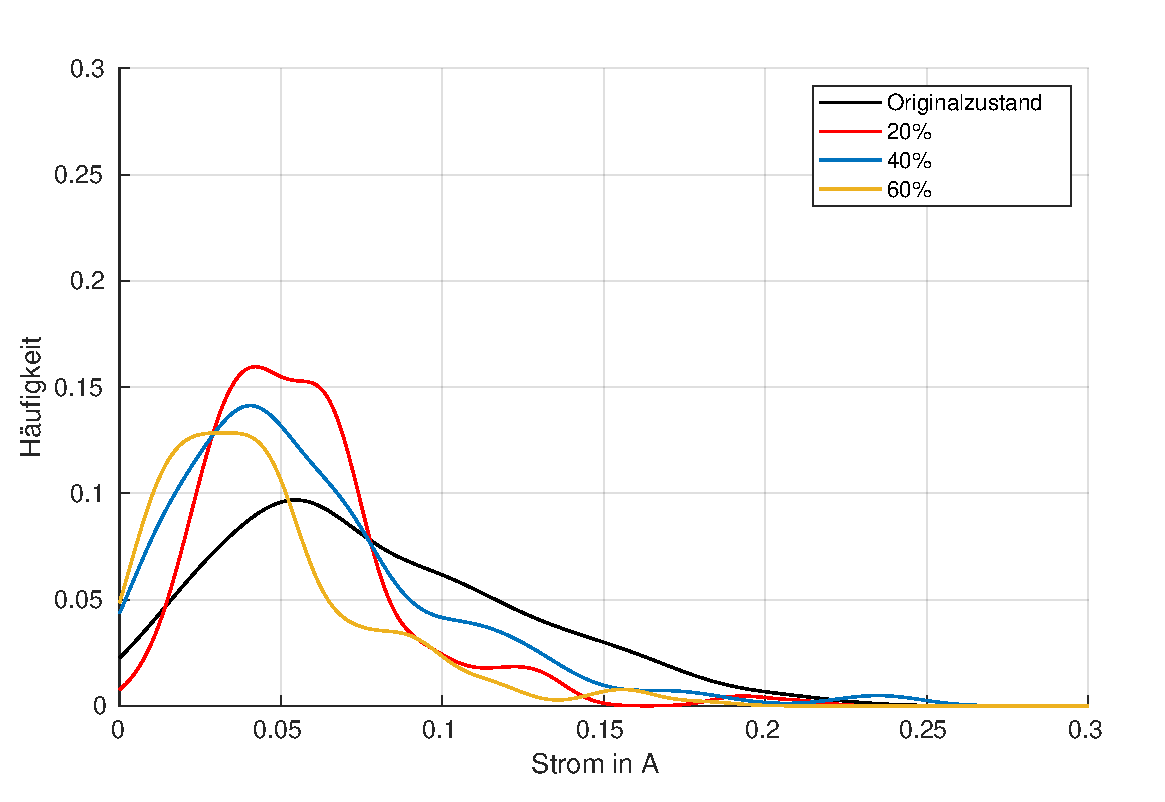
\includegraphics[width=\linewidth]{Bilder/links_Current_AnkleRoll_ohneM.pdf}
		%			\vspace{5pt}
	\end{subfigure}
	%		\hspace{20pt}
	%		\hfill
	\begin{subfigure}[c]{.9\linewidth}
		\centering
		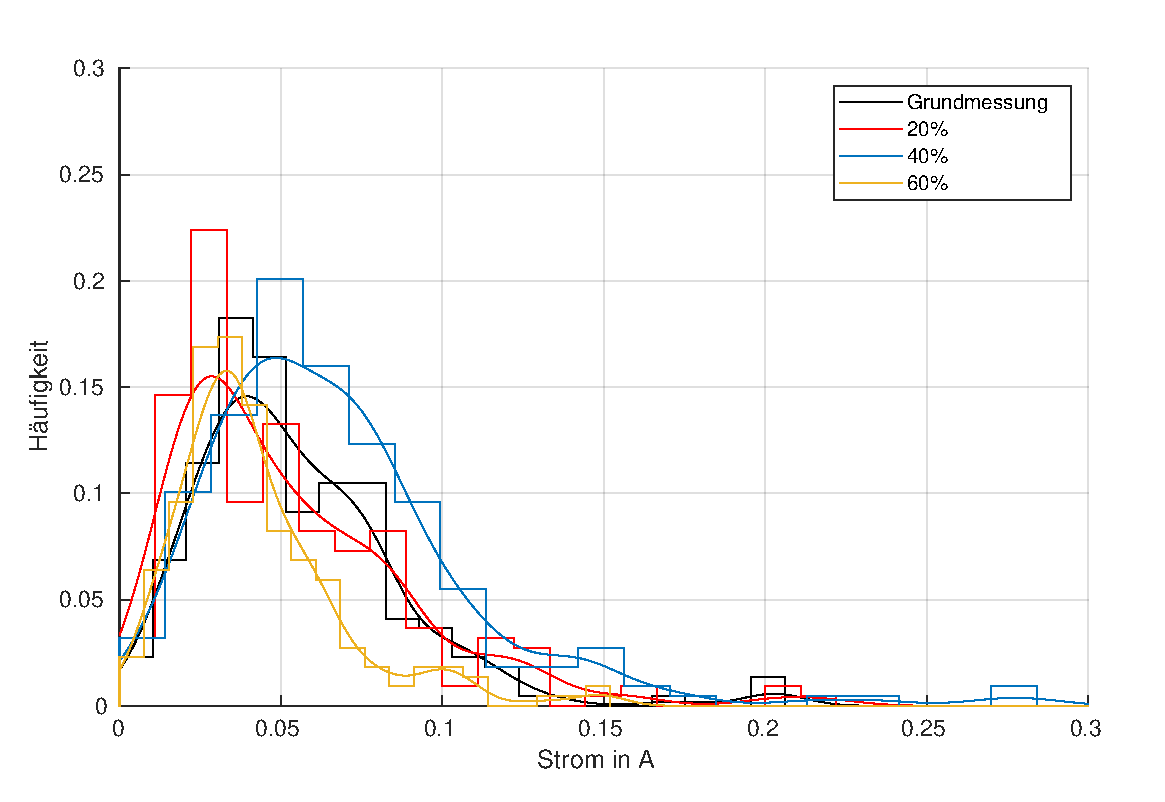
\includegraphics[width=\linewidth]{Bilder/links_Current_AnkleRoll_mitM.pdf}
		%			\vspace{5pt}
	\end{subfigure}
	%	\end{adjustwidth}
	\caption{AnkleRoll gemessener Strom im linken Fuß, Strom in Ampère aufgetragen auf die Häufigkeit. Das Histogramm wurde ergänzt durch eine Wahrscheinlichkeitsdichtefunktion. Der obere Graph sind die Aufnahmen ohne Magneten, der untere mit Magneten.} \label{AnkleRoll_Current_links}
\end{figure}
\begin{figure}[tb]
	\centering
	%	\begin{adjustwidth}{-0.2\linewidth}{-0.2\linewidth}
	%		\hspace{5pt}
	\begin{subfigure}[c]{.9\linewidth}
		\centering
		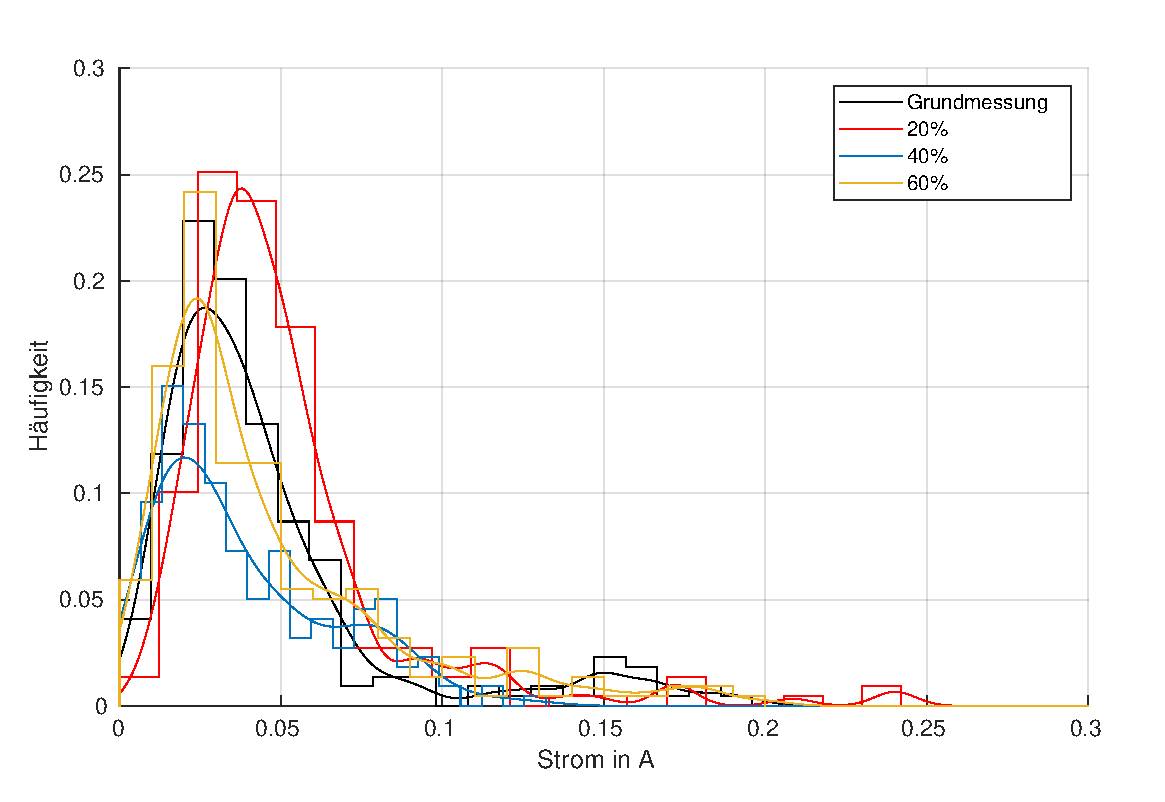
\includegraphics[width=\linewidth]{Bilder/rechts_Current_AnkleRoll_ohneM.pdf}
		\vspace{5pt}
	\end{subfigure}
	%		\hspace{20pt}
	\hfill
	\begin{subfigure}[c]{.9\linewidth}
		\centering
		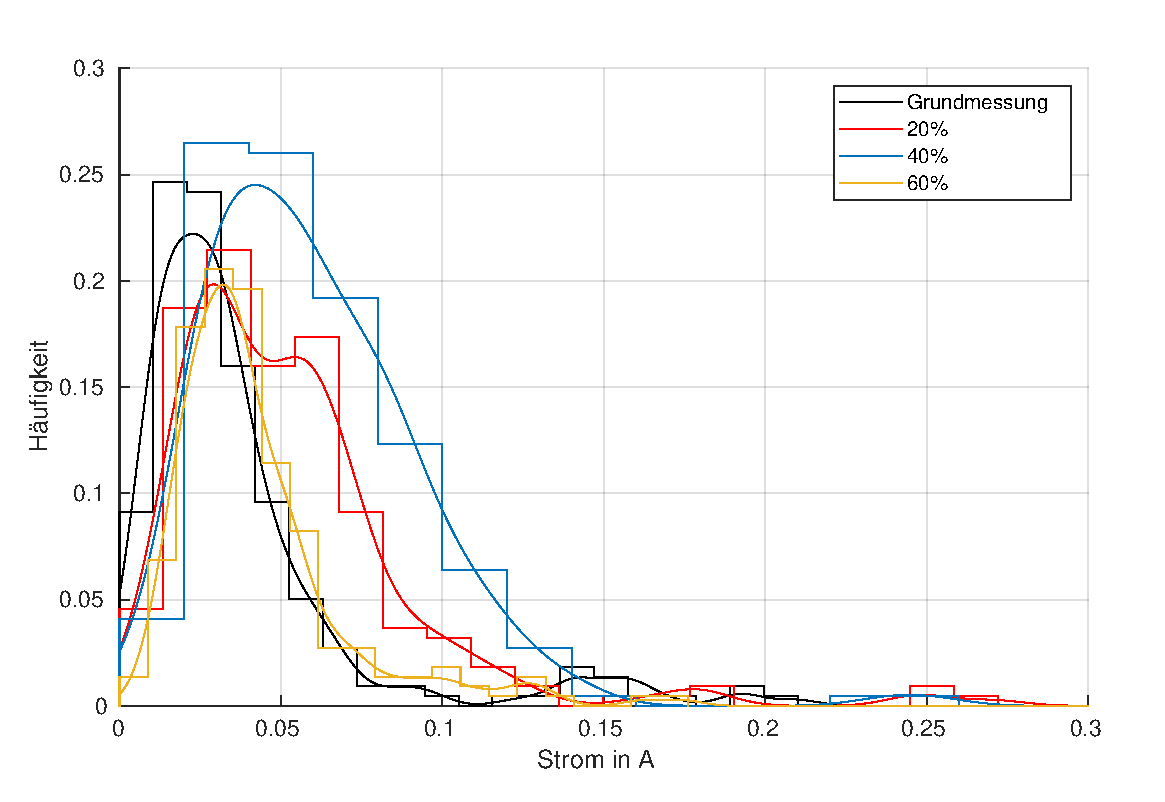
\includegraphics[width=\linewidth]{Bilder/rechts_Current_AnkleRoll_mitM.pdf}
		\vspace{5pt}
	\end{subfigure}
	%	\end{adjustwidth}
	\caption{AnkleRoll gemessener Strom im rechter Fuß, Strom in Ampère aufgetragen auf die Häufigkeit. Das Histogramm wurde ergänzt durch eine Wahrscheinlichkeitsdichtefunktion. Der obere Graph sind die Aufnahmen ohne Magneten, der untere mit Magneten.} \label{AnkleRoll_Current_rechts}
\end{figure}

%\subsection{Messungen von AnkleRoll zum Test}
%Die Messungen von LAnkleRoll und RAnkleRoll, zu sehen in Abb. \ref{hardware_llegjoint} und \ref{hardware_rlegjoint} wurden 20 mal wiederholt und mit den normalen Schuhen von Nao vollzogen. Dabei legte er in etwa eine Strecke von $0,8 \unit{m}$ auf der Rampe im flachen Zustand zurück. Insgesamt wurden alle verfügbaren Messwerte von AnkleRoll aufgezeichnet, das sind pro Aktor 6 Messwerte. Temperatur, Stiffness und Temperatur Status erwiesen sich als Konstant und daher nicht entscheidend, um einen Unterschied der Bodenbeschaffenheit oder Sohlen erkennen zu können. Stiffness ist immer auf $100\%$ während dem Gang. 
%Der Befehl für diesen Lauf war der moveTo() Befehl, welcher nicht weiter verändert wurde (kommt in den Theorieteil).
%
%
%In Abb. \ref{AnkleRoll_links_act} und \ref{AnkleRoll_rechts_act} sind die Messdaten von jeweils einem Fuß des Messwertes Position/Actuator abgebildet. Hier ist zu sehen, dass die Anfangswerte sich aufspalten, in positive und einmal in negative Winkelangaben. Dies ist der Tatsache geschuldet, dass die Funktion moveTo() per Zufall Nao mit dem linken oder mit dem rechten Fuß beginnen lässt. 
%
%Dies wurde für Abb. \ref{AnkleRoll_beide_act_sens_links_anfang} und \ref{AnkleRoll_beide_act_sens_rechts_anfang} sortiert. In ersterer Abbildung beginnt Nao mit dem linken Fuß. Da die Hüfte sich für den ersten Schritt nach rechts bewegen muss, verschiebt sich die Position beider Gelenke in die Negativrichtung, der Winkel wird absolut gemessen, wie in Abb \ref{hardware_llegjoint} und \ref{hardware_rlegjoint} zu sehen ist. 
%
%Außerdem sind in Abb. \ref{AnkleRoll_beide_act_sens_links_anfang} und \ref{AnkleRoll_beide_act_sens_rechts_anfang} neben den Messwerten von Position Actuator in schwarz auch die von Position Sensor in blau gezeigt. \textcolor{red}{Was diese beiden Messwerte genau unterscheidet und ob einer von moveTo() vorgegeben wird, ist noch zu entscheiden.} Der bedeutenste Unterschied ist zu Beginn der Aufnahmen. Die Position/Actuator Messung beginnt nahe 0, während Position/Sensor für den jeweiligen Fuß bei einem Wert über Null oder unter Null anfängt. 
%
%Es ist eindeutig zu erkennen, dass die Messungen erst nach der Sortierung des Anfangsschrittes ein regelmäßiges Bild ergeben. 
%
%Der Strom, welcher die Gelenke einsetzen müssen um das gewollte Ergebnis zu erzielen, scheint eine mögliche, vergleichbare Aufnahmegröße für unterschiedliche Sohlen und Umgebungen des Nao zu sein. In Abb. \ref{AnkleRoll_beide_current_links_anfang} und \ref{AnkleRoll_beide_act_sens_rechts_anfang} ist der Messwert Current aufgeteilt in Anfangsschritte gezeigt. Hier ist der Unterschied, mit welchem Fuß der erste Schritt gemacht wird, nicht so gravierend, wie bei den vorherigen Messwerten. Allerdings zeichnet sich eine Tendenz ab, dass der linke Fuß, hier in schwarz, einen höheren Strom beansprucht, als der rechte Fuß. Dies könnte dem beobachteten Fehlgang des Naos und dem zusätzlichen Geräusch bei jedem zweiten Schritt geschultet sein. Bei normaler Einstellung und ohne Korrektur würde dieser Nao einen Bogen nach rechts laufen. Um dies auszugleichen wurden bei moveTo() Anpassungen hinzugefügt.   
%
%\begin{figure}[tb]
%	\centering
%	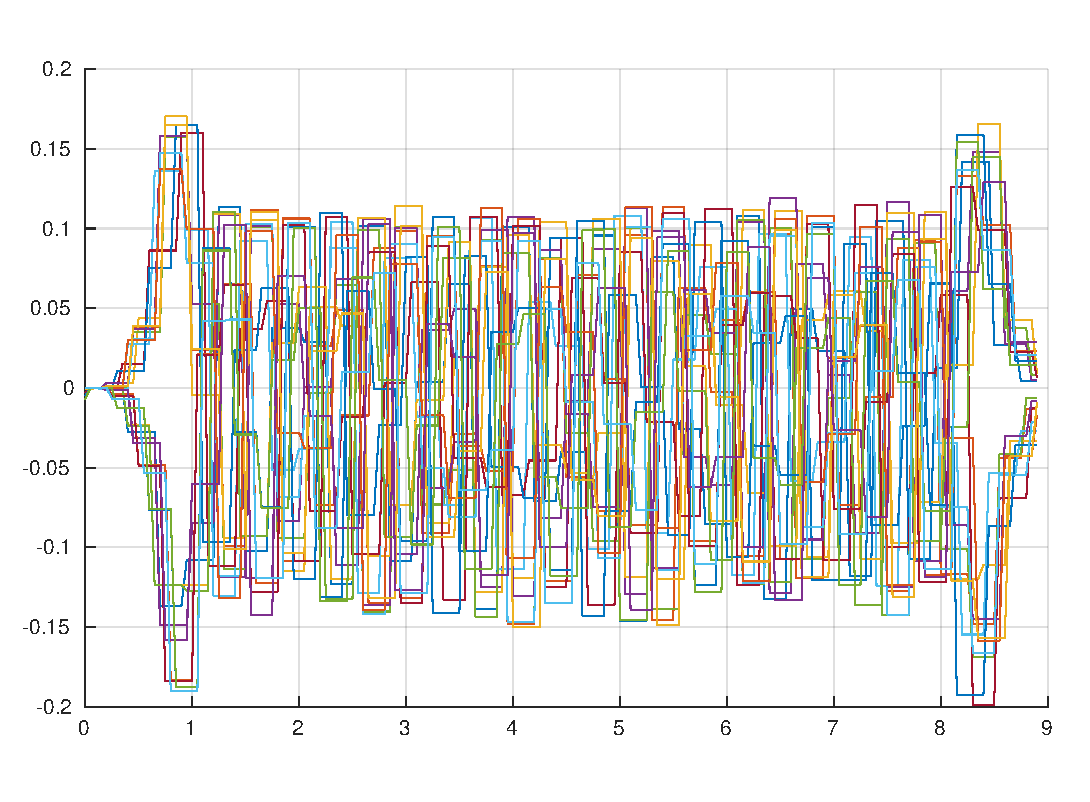
\includegraphics[width=1\linewidth]{Bilder/AnkleRoll_links_act.pdf}
%	\caption{AnkleRoll Messwert Position Actuator des linken Fußes}
%	\label{AnkleRoll_links_act}
%\end{figure}
%
%\begin{figure}[tb]
%	\centering
%	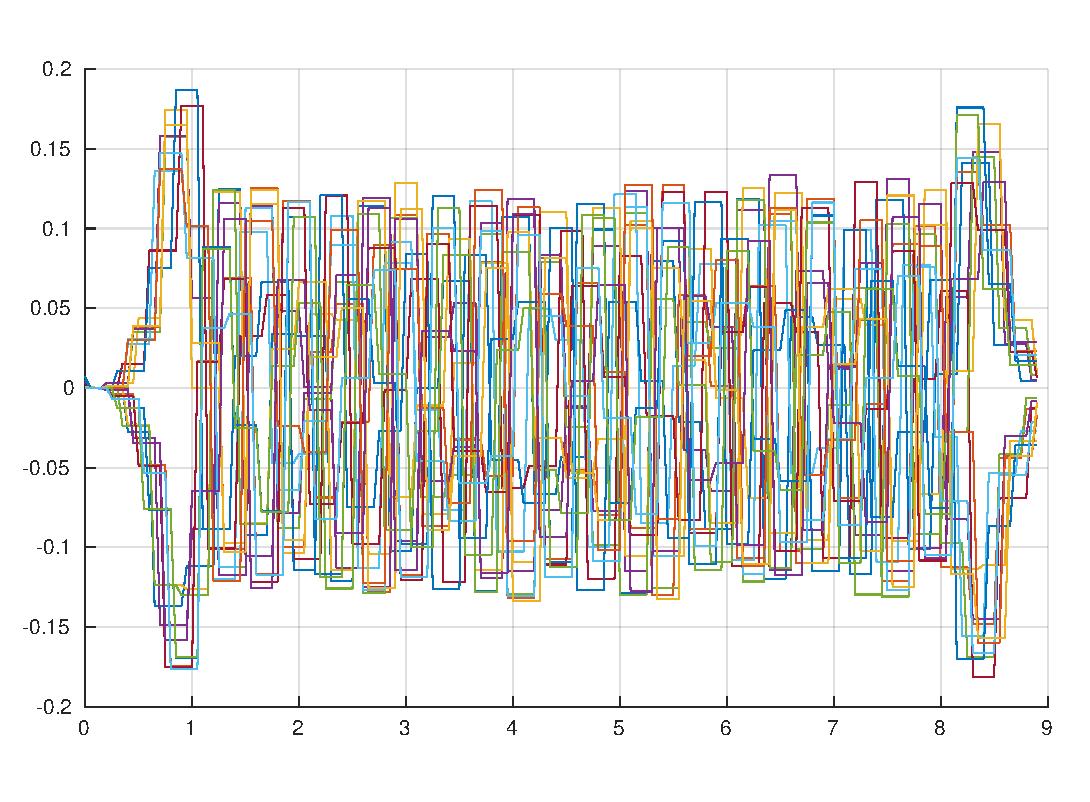
\includegraphics[width=1\linewidth]{Bilder/AnkleRoll_rechts_act.pdf}
%	\caption{AnkleRoll Messwert Position Actuator des rechten Fußes}
%	\label{AnkleRoll_rechts_act}
%\end{figure}
%\begin{figure}[tb]
%	\centering
%	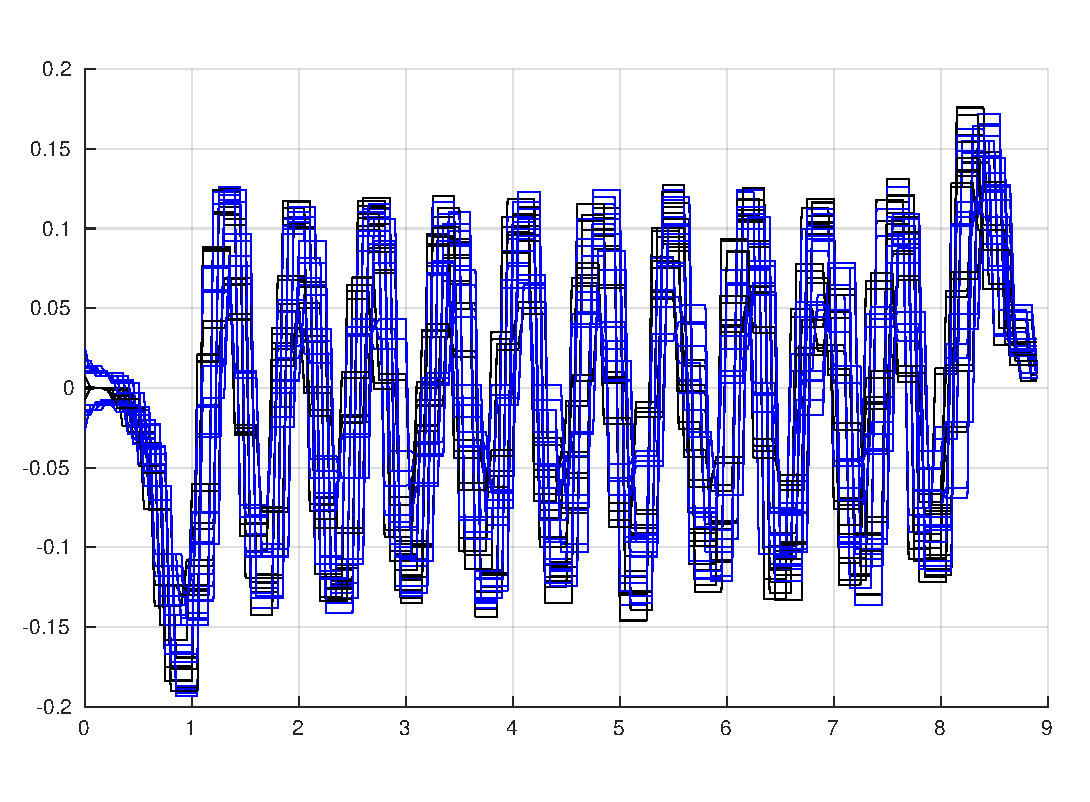
\includegraphics[width=1\linewidth]{Bilder/AnkleRoll_beide_act_sens_links_anfang.pdf}
%	\caption{AnkleRoll Aktoren beider Seiten mit dem Position/Actuator Messwert in schwarz und dem Position/Sensor Messwert in blau. Nao macht hier den ersten Schritt mit Links.}
%	\label{AnkleRoll_beide_act_sens_links_anfang}
%\end{figure}
%\begin{figure}[tb]
%	\centering
%	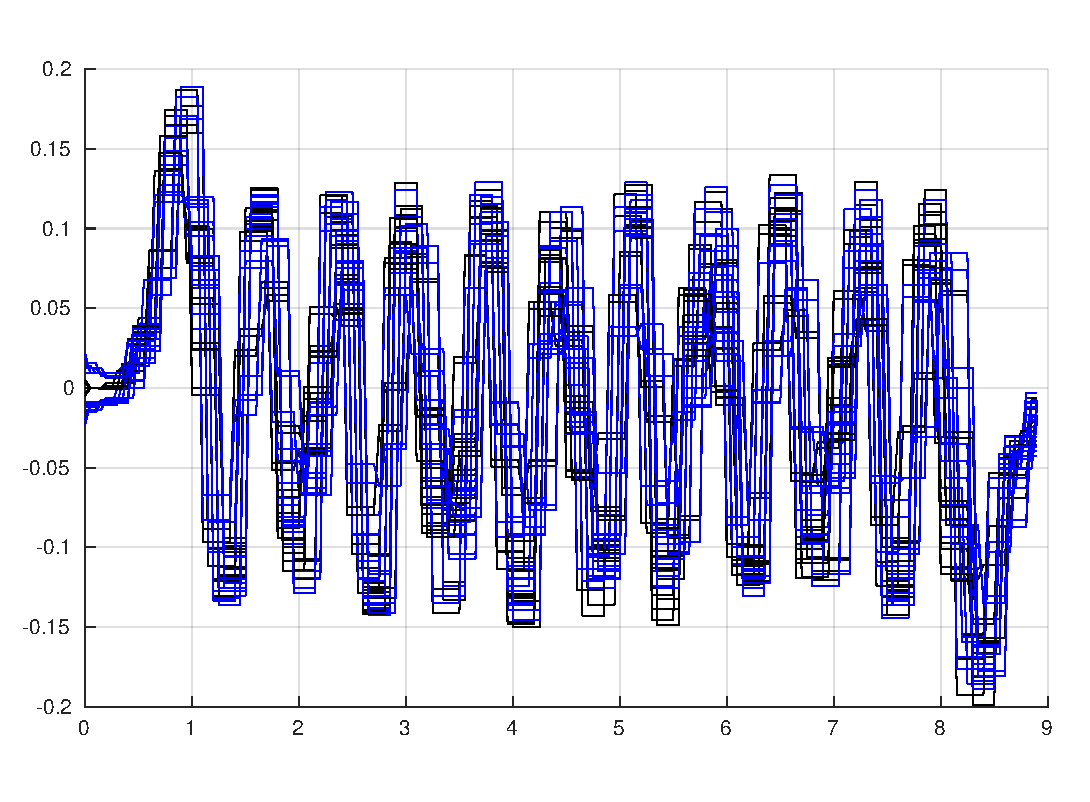
\includegraphics[width=1\linewidth]{Bilder/AnkleRoll_beide_act_sens_rechts_anfang.pdf}
%	\caption{AnkleRoll Aktoren beider Seiten mit dem Position/Actuator Messwert in schwarz und dem Position/Sensor Messwert in blau. Nao macht hier den ersten Schritt mit Rechts.}
%	\label{AnkleRoll_beide_act_sens_rechts_anfang}
%\end{figure}
%\begin{figure}[tb]
%	\centering
%	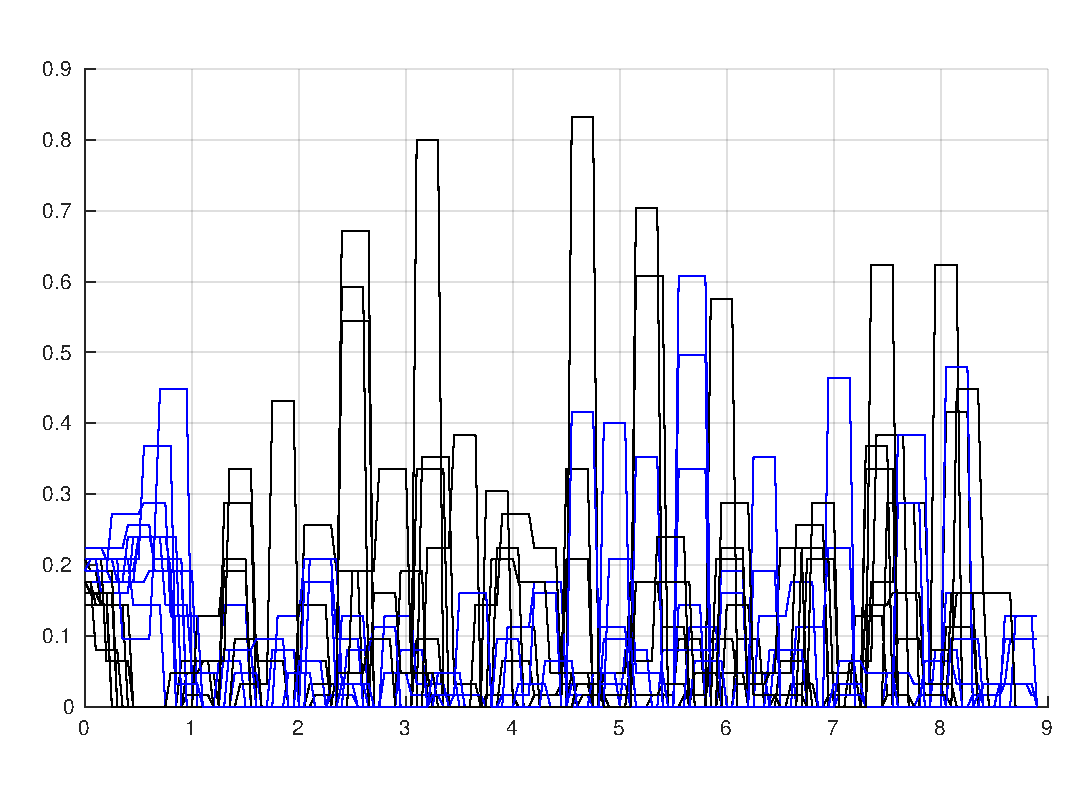
\includegraphics[width=1\linewidth]{Bilder/AnkleRoll_beide_current_links_anfang.pdf}
%	\caption{AnkleRoll Aktoren beider Seiten mit dem Current Messwert. Messwert Links ist in Schwarz, Messwert Rechts ist in Blau. Nao macht hier den ersten Schritt mit Links.}
%	\label{AnkleRoll_beide_current_links_anfang}
%\end{figure}
%\begin{figure}[tb]
%	\centering
%	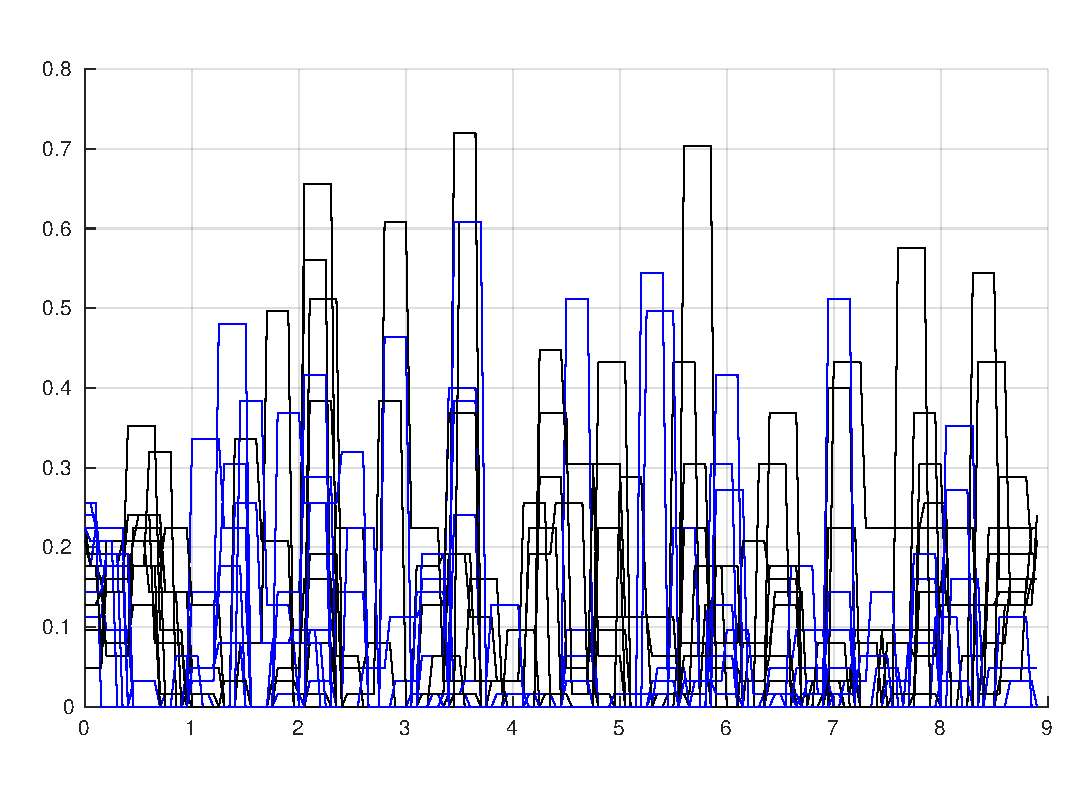
\includegraphics[width=1\linewidth]{Bilder/AnkleRoll_beide_current_rechts_anfang.pdf}
%	\caption{AnkleRoll Aktoren beider Seiten mit dem Current Messwert. Messwert Links ist in Schwarz, Messwert Rechts ist in Blau. Nao macht hier den ersten Schritt mit Rechts.}
%	\label{AnkleRoll_beide_current_rechts_anfang}
%\end{figure}

%%% Local Variables:
%%% mode: latex
%%% TeX-master: "main"
%%% End:

% Allgemeines zu diesem Nao (Vormessungen), Probleme der Messungenauigkeit
% Vergleichen der Messungen mit und ohne Magneten
%
\FloatBarrier
\newpage
\section{Fazit und Ausblick}
% zusammenfassen, was untersucht wurde
Diese Arbeit beschäftigte sich mit der Konstruktion eines Schuhs für den von Softbank Robotics hergestellten humanoiden Roboter NAO. Ziel war es, das bisher bereits vielseitig angewandte, aber noch nicht an Roboterfüßen verwendete MAP zu testen. Des Weiteren wurde eine Teststrecke mit der Möglichkeit Magneten anzubringen und verschiedene Winkel einzustellen gebaut, sowie die Stabilität des NAO erhöht. Außerdem sollten die Auswirkungen der neuen Lauffläche auf den Roboter getestet werden. 

% was waren die Ergebnisse
Zusammenfassend lässt sich, wie in Kapitel \ref{gleichgewicht} beschrieben, ein Zusammenhang zwischen erhöhter Stabilität, Magneten und CIP Anteil in den Sohlen erkennen. Die Prozentanteile, die verwendet wurden, unterscheiden sich sehr im Anteil von CIP und Gewicht. Die Reaktion auf das Magnetfeld waren für höhere Prozente ersichtlich, während der Originalschuh kaum Reaktion zeigte. Der Gang mit $20\,\%$ war ungewöhnlich stabil, sowohl mit als auch ohne Magneten. 

% welche Probleme gab es mit NAO
Während der Messarbeiten sind einige Problematiken in der Arbeit mit dem NAO Roboter herausgetreten. Bereits bei der Programmierung gab es Grenzen, da es sich um ein geschlossenes System handelt. NAO ist ein Roboter, der für das Arbeiten mit Kindern und Jugendlichen konzipiert wurde und ist hauptsächlich ein Vorführungsobjekt. Die Gangarten sind begrenzt und ein Ausgleichssystem, welches dem Roboter eine Rückkopplung für Umgebungserkennung gewährleisten würde, lies sich nicht mit der Aufnahme von Messdaten vereinbaren. Dazu hätten externe Sensoren und weitere Geräte angeschlossen werden müssen. Hinzu kommt, dass NAOs Sensoren nicht exakt genug sind, wie bereits in \cite{pressure_shoe} beschrieben. Dies erschwerte eine genauere Bestimmung von Stabilität und Aufwand. Des Weiteren konnte NAO zu Beginn bereits nicht geradeaus laufen. Dies musste manuell ausgeglichen werden und führte dazu, dass NAO u.U. nicht exakt dieselbe Strecke zurücklegte. Und schließlich begann der \texttt{moveTo()} Befehl per Zufall die Bewegung mit dem linken oder rechten Fuß. Dies hat zur Folge, dass die Aktoren unterschiedliche Ausgaben zu gleichen Zeiten haben und könnte die Mittelwerte verfälscht haben, welche zum Vergleich erstellt wurden. 

Da eine höhere Stabilität feststellbar war, siehe hierzu Abb. \ref{fwhm}, könnte diese Art der Sohlenentwicklung interessant sein für künftige Konstruktionen in der Robotik. Außerdem ist die durch diese Arbeit entstandene Rampe vor allem für künftige Testläufe mit diversen Laufrobotern und Softrobotern geeignet. 
% ist es sinnvoll weiter an MAP Sohlen zu arbeiten. (Rampe erwähnen)

%%% Local Variables:
%%% mode: latex
%%% TeX-master: "main"
%%% End:
%was nicht funktioniert hat (auch, weil Zeit gefehlt hat)
%
\FloatBarrier
\newpage
\section{Anhang} \label{Anhang}
	\begin{python} [caption={Pythonprogramm für Messaufnahmen}, label=Messungscode]
		# ! /usr/bin/env python
		# -*- encoding: UTF-8 -*-
		
		"""Example: Use getData Method to Use FSR Sensors"""
		
		import qi
		import argparse
		import sys
		import time
		import csv
		import re
		import shutil
		from tempfile import mkstemp
		import os
		
		def sed(pattern, replace, source, dest=None, count=0):
			"""Reads a source file and writes the destination file.
			
			In each line, replaces pattern with replace.
			
			Args:
			pattern (str): pattern to match (can be re.pattern)
			replace (str): replacement str
			source  (str): input filename
			count (int): number of occurrences to replace
			dest (str):   destination filename, if not given, source will be over written.
			"""
			
			fin = open(source, 'r')
			num_replaced = count
			
			if dest:
				fout = open(dest, 'w')
			else:
				fd, name = mkstemp()
				fout = open(name, 'w')
			
			for line in fin:
				out = re.sub(pattern, replace, line)
				fout.write(out)
				
				if out != line:
				num_replaced += 1
				if count and num_replaced > count:
				break
			try:
				fout.writelines(fin.readlines())
			except Exception as E:
				raise E
			
			fin.close()
			fout.close()
			
			if not dest:
				shutil.move(name, source)
		
		
		def zeilen_aufteilen(file):
			sed(',platzhalter,', '\n', file)
			sed(',platzhalter', '', file)
		
		
		def recordData(memory_service):
			""" Get pressure sensor data from ALMemory
			Returns a matrix of values
			
			"""
			print "Recording data..."
			data = list()
			for range_counter in range(1, 230):
				#Gyroscope
				GyrX = memory_service.getData("Device/SubDeviceList/InertialSensor/GyroscopeX/Sensor/Value")
				GyrY = memory_service.getData("Device/SubDeviceList/InertialSensor/GyroscopeY/Sensor/Value")
				data.append(GyrX)
				data.append(GyrY)
				
				# Adding the summary of the FSR
				LFsrTw = memory_service.getData("Device/SubDeviceList/LFoot/FSR/TotalWeight/Sensor/Value")
				RFsrTw = memory_service.getData("Device/SubDeviceList/RFoot/FSR/TotalWeight/Sensor/Value")
				
				LFcopX = memory_service.getData("Device/SubDeviceList/LFoot/FSR/CenterOfPressure/X/Sensor/Value")
				LFcopY = memory_service.getData("Device/SubDeviceList/LFoot/FSR/CenterOfPressure/Y/Sensor/Value")
				RFcopX = memory_service.getData("Device/SubDeviceList/RFoot/FSR/CenterOfPressure/X/Sensor/Value")
				RFcopY = memory_service.getData("Device/SubDeviceList/RFoot/FSR/CenterOfPressure/Y/Sensor/Value")
				data.append(LFsrTw)
				data.append(RFsrTw)
				data.append(LFcopX)
				data.append(LFcopY)
				data.append(RFcopX)
				data.append(RFcopY)
				
				# LeftAnkleRoll
				PosAct = memory_service.getData("Device/SubDeviceList/LAnkleRoll/Position/Actuator/Value")
				PosSens = memory_service.getData("Device/SubDeviceList/LAnkleRoll/Position/Sensor/Value")
				ElectrSens = memory_service.getData("Device/SubDeviceList/LAnkleRoll/ElectricCurrent/Sensor/Value")
				data.append(PosAct)
				data.append(PosSens)
				data.append(ElectrSens)
				
				# RightAnkleRoll
				PosAct = memory_service.getData("Device/SubDeviceList/RAnkleRoll/Position/Actuator/Value")
				PosSens = memory_service.getData("Device/SubDeviceList/RAnkleRoll/Position/Sensor/Value")
				ElectrSens = memory_service.getData("Device/SubDeviceList/RAnkleRoll/ElectricCurrent/Sensor/Value")
				data.append(PosAct)
				data.append(PosSens)
				data.append(ElectrSens)
				
				# LeftAnklePitch
				PosAct = memory_service.getData("Device/SubDeviceList/LAnklePitch/Position/Actuator/Value")
				PosSens = memory_service.getData("Device/SubDeviceList/LAnklePitch/Position/Sensor/Value")
				ElectrSens = memory_service.getData("Device/SubDeviceList/LAnklePitch/ElectricCurrent/Sensor/Value")
				data.append(PosAct)
				data.append(PosSens)
				data.append(ElectrSens)
				
				# RightAnklePitch
				PosAct = memory_service.getData("Device/SubDeviceList/RAnklePitch/Position/Actuator/Value")
				PosSens = memory_service.getData("Device/SubDeviceList/RAnklePitch/Position/Sensor/Value")
				ElectrSens = memory_service.getData("Device/SubDeviceList/RAnklePitch/ElectricCurrent/Sensor/Value")
				data.append(PosAct)
				data.append(PosSens)
				data.append(ElectrSens)
				
				data.append('platzhalter')
				time.sleep(0.05)
			return data
		
		
		def count_files():
			counter = 1
			# str.zfill schreibt vor, wie lang die Zahl mit Nullen davor sein soll. also zfill(3) ist 3 Zahlen lang.
			filename = 'measurement' + str(counter).zfill(3) + '.csv'
			
			# Wenn das file nicht exisiert, erstelle measurement001.csv
			while os.path.exists(filename):
				counter = counter + 1
				filename = 'measurement' + str(counter).zfill(3) + '.csv'
			create_file(filename)
			return filename
		
		
		def create_file(filename):
			with open(filename, "w") as f:
				pass
		
		
		def main(session):
			"""
			This example uses the getData method to use FSR sensors.
			"""
			# Get the ALProxy ALMemory and ALMotion
			from naoqi import ALProxy
			memory_service = session.service("ALMemory")
			motion = ALProxy("ALMotion", "nao.local", 9559)
			
			# wake up nao
			motion.wakeUp()
			
			motion.moveInit()
			motion.post.moveTo(0.85, -0.10, -0.25, [["MaxStepFrequency", 0.0]])
			
			data = recordData(memory_service)
			filename = count_files()
			
			output = os.path.abspath(filename)
			with open(output, "wb") as file:
				writer = csv.writer(file, delimiter=',')
				writer.writerow(data)
			zeilen_aufteilen(output)
			print "Results written to", output
			# go back to crouch position and sleep
			motion.rest()
			
		
		if __name__ == "__main__":
			parser = argparse.ArgumentParser()
			parser.add_argument("--ip", type=str, default="127.0.0.1",
			help="Robot IP address. On robot or Local Naoqi: use '127.0.0.1'.")
			parser.add_argument("--port", type=int, default=9559,
			help="Naoqi port number")
			
			args = parser.parse_args()
			session = qi.Session()
			try:
				session.connect("tcp://" + args.ip + ":" + str(args.port))
			except RuntimeError:
				print ("Can't connect to Naoqi at ip \"" + args.ip + "\" on port " + str(args.port) + ".\n"
				"Please check your script arguments. Run with -h option for help.")
			sys.exit(1)
			main(session)	
	\end{python}
Der Programmcode \ref{Messungscode} kann in mehrere Funktionen aufgeteilt betrachtet werden. Die Funktion \texttt{sed} ist aus (cite) entnommen und funktioniert wie die gleichnamige Funktion unter der Linux-Bash. Sie wird benötigt, um nach jedem Durchgang der Messschleife in \texttt{recordData} eine neue Zeile in die CSV Datei zu schreiben. Dies geschieht durch die Funktion \texttt{zeilen\_aufteilen}. \texttt{recordData} wurde aus den Beispielen der NAO Dokumentation (cite) entnommen und angepasst, sodass am Ende jeder Zeile von \texttt{data} ein Platzhalter eingefügt wird und alle gewünschten Sensoren abgegriffen werden. Die Funktion \texttt{count\_files} sorgt dafür, dass keine vorhandenen Messungen überschrieben werden und jede Messdatei eine fortlaufende Nummerierung erhält. 

In der \texttt{main} Funktion werden ALMemory und ALMotion geladen, und der Gang einschließlich des Abgreifens der Sensorwerte ausgeführt. Die Ausgabe der Messwerte während dem Gang ist nur möglich durch den Präfix \texttt{post} vor \texttt{moveTo}.

Abschließend dient die letzte \texttt{if}-Abfrage zur Verbindung mit NAO, allerdings nur, wenn dieses Pythonprogramm selbst auf dem NAO liegt. Die Methode \texttt{post} sowie die Aufnahme der Sensoren während dem Lauf der Methode \texttt{moveTo} funktionieren nur lokal, deshalb ist es in diesem Fall nicht möglich, das Programm von dem eigenen Rechner aus zu starten. Mit anderen Methoden wäre eine Programmaufrufung über eine Wlan Verbindung durchaus möglich. Um Programme direkt auf dem NAO zu starten, wird eine \texttt{ssh}-Verbindung hergestellt und darüber dann \texttt{python} ausgeführt.
		
%%% Local Variables:
%%% mode: latex
%%% TeX-master: "main"
%%% End:

\FloatBarrier
\newpage
\clearpage	
%\thispagestyle{empty}
\printbibliography

\end{document}

%%% Local Variables:
%%% mode: latex
%%% TeX-master: "main"
%%% End: